\chapter{Surface Inpainting}

\section{Introduction}

In principle, surface inpainting refers to the completion or recovery of
missing shape geometry based on the shape information that is currently
available. The most prominent application of surface inpainting is mesh repair.
Due to factors such as occlusions, low reflectance, and quality limitations of
scanning equipments, 3D models generated from range scanners often contain
holes that need to be filled; sometimes the source model itself has missing
pieces and requires digital repair to attain a complete model. Another common
application of surface inpainting is to remove geometric features because of
shape editing needs. This is achieved by replacing the unwanted shape regions
with inpainting patches.

From the statistical point of view, surface inpainting can be viewed as an
estimation problem which infers the missing geometry from the observable shape,
and the inpainting result is determined by the statistical model we have
adopted. Generally speaking, there is no universally acceptable ``correct''
estimation; selecting the best inpainting is usually subjective or dependent on
the requirement of downstream applications.

Most existing surface inpainting methods tackle the problem only in
the mesh domain. These methods typically employ some geometric
constraints as heuristics to ensure that the obtained inpainting patch
is visually pleasing and blend naturally with its neighboring
geometry. The primary issue of geometry-constrained inpainting is that
these methods only utilize the shape information in the vicinity of
missing regions rather than consider the model in question in its
entirety.

Our new surface inpainting method documented is inspired
by the theory of sparse signal recovery and compressed sensing. The
intuition is that for a meaningful 3D model, even though its global
geometry is a high-dimensional signal, it most likely has a
low-dimensional intrinsic structure. That is to say, the
high-dimensional shape signal actually lives in a low-dimensional
subspace, which can be captured by a sparse coefficient representation
in some transformed (e.g., Fourier) domains. In another word, the
coordinate function of a shape with $N$ vertices can be decomposed as or
well approximated by the linear combination of $k\ll N$ basis signals.
According to the compressed sensing theory, the sparse coefficient
representation can be recovered from partial measurements as long as
the signal is sufficiently sparse and the sensing matrix satisfies
certain properties~\cite{Candes2006}.

The critical idea of our new inpainting algorithm is to estimate the
spectral coefficient representation of the shape geometry from partial
observations by imposing sparsity constraints on the reconstructed
coefficients, exploiting the fact that most 3D models are highly
compressible with respect to their Laplacian eigenfunctions~\cite{Karni2000}.
To the best of our knowledge, the utility of Laplacian eigenbasis towards
the shape inpainting application has not yet been explored in the past.
The estimation problem can be formulated with a data term strongly emphasizing
fidelity to the observations and a penalty term constraining sparsity of the
representation. Thus, the surface inpainting could be transformed to a
sparse signal recovery problem and can be solved by either $l_0$ or
$l_1$ optimization techniques. Such effort represents our first
attempt towards technical innovation.

The primary advantage of our method is that the inpainting takes into
account the information of all the remaining shape instead of only the
vicinity of missing regions. Rather than directly estimating the
missing geometry, we actually estimate the reconstruction coefficients
of the whole original shape. Since the mesh Laplacian basis functions are
smooth and have global support, the reconstructed inpainting shape is
naturally smooth and globally coherent with a simple intrinsic
structure.

The main contributions of this work are:
\begin{itemize}

\item We introduce a new surface inpainting framework based on
  representations in the transformed domain and sparsity constraints
  on reconstruction coefficients. This framework can make use of the
  information of the whole remaining shape and inpainting results
  tend to be simple and globally coherent.

\item We study the sparsity of 3D shapes with respect to their
  Laplacian eigenbases and show their effectiveness in surface
  inpainting.

\item We demonstrate the high performance of our inpainting method
  with several examples in hole filling and mesh editing.

\end{itemize}


\section{Background}
\label{sec:related}

\subsection{Surface Inpainting}

Many methods have been proposed in the research literature dealing
with the general problem of surface inpainting, bearing different
names such as hole filling, mesh completion, and surface restoration.
We refer readers to~\cite{Attene2013} for a recent survey of popular
algorithms for hole filling and mesh completion.

One simple approach for surface inpainting is by filling the missing
region with an inpainting patch that interpolates the surrounding
geometry. The interpolating patch may be generated with simple
polynomial functions~\cite{Wang2007}, triangular
B-splines~\cite{Pfeifle1996}, or radial basis
functions~\cite{Branch2006}, and are generally smooth and continuous
across the boundaries. The interpolation-based approaches, however,
only work well with disk-like holes and are not suitable for filling
regions with complex boundaries.

Typical mesh-based hole filling algorithms have two steps: (1) Find an
initial triangulation of the missing region defined by the hole
boundary; (2) Optimize the inserted mesh to improve its fairness and
coherence with surrounding shapes. In \cite{Liepa2003}, Liepa
performed hole triangulation with a dynamic programming technique
taking into account the dihedral angles and areas of the created
triangles. The inserted mesh is then optimized with Laplacian
smoothing to improve fairness. In \cite{Zhao2007}, surface holes are
patched by an advancing-front mesh generation method, and the vertex
positions are optimized by solving a Poisson equation based on the
desirable triangle normals computed from boundary vertices. In \cite{Bac2008},
the coordinates of the inserted vertices are optimized by minimizing the
discrete thin-plate energy.
In \cite{Li2010}, \cite{Wang2012} and \cite{Ngo2013}, complex holes are
first partitioned into sub-holes by feature curves extended from the
existing parts; typical hole-filling then can be performed on these
sub-holes which are much more planar.

Another class of inpainting algorithms are based on variational
methods. The basic idea is to iteratively evolve the inpainting shape
by optimizing a functional that constrains certain geometric
properties of the inserted mesh, e.g., positions, areas, tangency, and
curvatures. In \cite{Pernot2006}, Pernot et al. developed a hole
filling algorithm which minimizes the variational involving curvature
between the surrounding and inpainted geometry. In
\cite{Caselles2008}, the completing surface is chosen such that a
power of the mean curvature is minimized. In \cite{Clarenz2004},
Clarenz et al. proposed a shape restoration algorithm by computing the
$l_2$-gradient flow of the Willmore energy which ensures the
continuity of the normal field.

Finally, a lot of mesh inpainting methods are exemplar-based. In
\cite{Kraevoy2005}, Kraevoy and Sheffer introduced an algorithm for
mesh completion by mapping the incomplete mesh with a template model.
Context-based surface completion methods like \cite{Sharf2004} and \cite{Park2005}
fill holes by importing patches from similar regions and adapt them
to the hole regions via shape deformation. A coherence objective can be imposed
such that every local neighborhood of the filled mesh is similar to some local
neighborhood from the input mesh~\cite{Harary2014}.

\subsection{Sparse Signal Recovery and Inpainting}

Recent years have witnessed a surge in the research of sparsity-based
signal recovery. The fundamental idea is that a sufficiently sparse
signal can be reliably reconstructed from partial measurements by
exploiting the sparsity cue.

Sparse signal recovery has seen most success in compressed sensing
applications, where the measurement/sensing matrix is typically chosen
as a normalized random matrix which satisfies the restricted isometry
property with high probability. For the inpainting problem, the
measurement is expressed as a mask matrix, which is not strictly a
valid compressed sensing process. Nonetheless, we can still take
advantage of the sparsity constraints to recover the original signals
in many situations.

For image inpainting and restoration tasks, many algorithms based on
 sparse representation have been published. In \cite{Guleryuz2006} and
\cite{Guleryuz2006a}, Guleryuz proposed an algorithm for image
recovery based on adaptive sparse representation. In \cite{Elad2005},
images are decomposed into texture and cartoon components, each of
which is sparse with respect to a particular dictionary; the missing
parts then can be easily reconstructed. In \cite{Fadili2005} and
\cite{Fadili2009}, Fadili et al. formulated image inpainting as a
maximum-likelihood estimation problem with a sparsity-promoting prior
penalty imposed on the reconstructed coefficients. A similar
formulation is proposed in \cite{Cai2008} where images have sparse
framelet representations and the incomplete image can be restored via
an iterative shrinkage algorithm. This formulation balances the
sparsity of coefficients, fidelity to the existing data, as well as
the smoothness of the solution. In \cite{Ogawa2011}, Ogawa et al.
proposed an image recovery algorithm based on sparse representation,
in which the low-dimensional subspaces optimal for targeted missing
textures are adaptively selected.

There have been very few works on the sparsity-induced recovery of
signals defined on graphs. In \cite{Zhu2012}, Zhu
and Rabbat proposed to use the dictionary of graph Laplacian
eigenfunctions to recover smooth and sparse graph signals and applied them
to the reconstruction of wireless sensor networks data from partial
node readings. To the best of our knowledge, our method is the first
of such attempts to tackle the problem of geometry
inpainting/completion via sparse signal recovery.

\section{Variational Inpainting Model}
\label{sec:inpaint:model}

The problem of mesh signal inpainting can be stated as follows.
Consider a triangle mesh $M=\{V,E\}$ with $n$ vertices, where $V$ and
$E$ denote the set of vertices and edges, respectively. Let
$\mathbf{f}\in\mathbb{R}^n$ be a vector signal defined on the mesh
vertices. Assume the signal values at a subset of vertices $V'\subset
V$ are already known, the goal of inpainting is to compute a
reasonable estimate of the remaining signal values at $V - V'$. For
the problem of inpainting surface geometry, the mesh signal is the
coordinate function and the unknown parts correspond to surface holes.

Assume the number of known vertices is $|V'|=n'$. We can define the
$n' \times n$ projection matrix $P$ as
\begin{equation}
P(i,j) = \left\{
    \begin{array}{l l}
    1 & \quad \text{if $v_j$ is the $i$th element of $V'$}\\
    0 & \quad \text{otherwise.}
    \end{array}\right.
\end{equation}

Denote the observable parts of $\mathbf{f}$ to be $\mathbf{f'} \in
\mathbb{R}^{n'}$, which should satisfy $\mathbf{f}' = P\mathbf{f}$,
the general inpainting problem can be formulated as a constrained
optimization problem
\begin{equation}
\label{eq:inpainting}
\hat{\mathbf{f}} = \arg\min_{\mathbf{f}} \text{Pr}(\mathbf{f}) \quad \text{s.t.} \quad \|P\mathbf{f} - \mathbf{f'}\|_2^2 < \epsilon,
\end{equation}
or equivalently as a penalized maximum-likelihood estimation problem
\begin{equation}
\label{eq:inpainting2}
\hat{\mathbf{f}} = \arg\min_{\mathbf{f}} \text{Pr}(\mathbf{f}) + \lambda \|P\mathbf{f} - \mathbf{f}'\|_2^2,
\end{equation}
where the data term $\|P\mathbf{f} - \mathbf{f}'\|_2^2$ emphasizes
fidelity to the available observations, while $\text{Pr}(\hat{f})$ is
a prior regularizing certain properties of the reconstructed signal.

Traditionally, priors are chosen to optimize the fairness of the
inserted mesh or its coherence with the surrounding geometry. For
example, a commonly-adopted prior for surface optimization is
$\text{Pr}(\mathbf{f})=\|L\mathbf{f}\|_2^2$ which aims to maximize the
smoothness of the estimated signal, generating the so-called
\emph{least-squares meshes} \cite{Sorkine2004}. Here $L$ is the
Laplace operator of the shape.

Instead of computing the approximate signal $\hat{\mathbf{f}}$ in the
mesh domain directly, we may first estimate the original signal's
representation in some transformed domains. Consider a dictionary $D$
of $m$ atoms, where each atom is an elementary signal defined on the
mesh; written in the matrix form,
$D=(\mathbf{d_1},\ldots,\mathbf{d_m}), \mathbf{d_i}\in
\mathbb{R}^{n\times 1}$. The original signal $f$ may be represented as
the linear combination of columns in $D$
\begin{equation}
\mathbf{f} = D\mathbf{\alpha} = \sum_{i=1}^{m}\alpha_i\mathbf{d_i},
\end{equation}
where $\mathbf{\alpha} = (\alpha_1,\ldots,\alpha_m)^T$ is the
coefficient representation of $\mathbf{f}$ w.r.t. the dictionary $D$.

Obviously, if we can estimate the coefficient representation of the
whole original signal from partial measurements $\mathbf{f}'$, then we
also obtain an inpainting of the missing signal values. If we know in
advance that the coefficients of representation of $\mathbf{f}$
satisfy certain statistical properties, we can estimate the
coefficients by imposing a prior on $\mathbf{\alpha}$
\begin{equation}
\label{eq:inpainting3}
\hat{\mathbf{\alpha}} = \arg\min_{\mathbf{\alpha}} \text{Pr}(\mathbf{\alpha}) \quad \text{s.t.} \quad \|PD\mathbf{\alpha} - \mathbf{f'}\|_2^2 < \epsilon,
\end{equation}
The complete original signal can then be estimated as
$\hat{\mathbf{f}}=D\mathbf{\hat{\alpha}}$.


\section{Sparsity-Based Surface Inpainting}

The fundamental idea of our sparsity-based surface inpainting method is that,
for most natural shapes, although the surface geometry is a high-dimensional
signal, it actually lives in a low-dimensional subspace and has a sparse
representation in some transformed domains. Hence, we can set the sparsity of
coefficients as the prior in Eq.~\ref{eq:inpainting3} to estimate the
coefficient representation of the global shape and recover the missing
geometry. As long as the ``complexity'' of the original shape is much smaller
than the number of available observations, we have a good chance to obtain a
plausible restoration.

In this section, we first discuss the sparsity of shape geometry w.r.t. the
mesh Laplacian eigenbasis, demonstrating the potentials of Laplacian
eigenfunctions for sparsity-based geometry processing. Then we propose a
sparsity-constrained formulation for the problem of surface inpainting with
known connectivity. Finally, we extend our inpainting method to hole
filling-in where mesh connectivity is nonexistent in the missing regions in
the first place.

\subsection{Laplacian Eigenbasis}

For a discrete mesh, its graph Laplacian matrix $L$ is typically
defined as
\begin{equation}
L(i,j) = \left\{
    \begin{array}{l l}
    1 & \quad \text{if $(v_i, v_j) \in E$} \\
    0 & \quad \text{otherwise.}
    \end{array}\right.
\end{equation}

The set of eigenfunctions of L, $\Phi = \{\phi_i\}_{i=1}^n$, are commonly
referred to as Laplacian eigenbasis or manifold harmonic basis
(MHB)~\cite{Vallet2008}. The Laplacian eigenfunctions are analogous to
the classic Fourier basis in Euclidean space and have the following similar
properties:
\begin{itemize}
\item Functions in $\{\phi_i\}$ all have global support on the mesh.
\item Functions in $\{\phi_i\}$ exhibit wave-like periodical
  oscillations on the mesh with different frequencies corresponding to
  the eigenvalues $\{\lambda_i\}$.
\item $\{\phi_i\}$ form a complete, orthonormal basis of the
  square-integrable function space $L^2(M)$ defined on the mesh.
\item $\{\phi_i\}$ induce a spectral transform: Any signal $f\in
  L^2(M)$ have a unique decomposition w.r.t. $\{\phi_i\}$
      $$f=\sum_{k=1}^n \tilde{f}(k) \phi_k = \sum_{k=1}^n \langle f,\phi_k \rangle \phi_k,$$
      in which $\tilde{f}(k)$ denotes the $k$th spectral/Fourier
      coefficient.
\end{itemize}

The aforementioned attractive properties make Laplacian eigenfunctions
potentially efficient for representing shape signals defined on
meshes. In \cite{Karni2000}, Karni and Gotsman utilized the truncated
spectral coefficients for compressed representation of mesh geometry, which
is very similar to the JPEG format for image compression.
In \cite{Ben-Chen2005}, Ben-chen and Gotsman further proved that the
Laplacian eigenbasis is the optimal basis for mesh compression in the
mean square error (MSE) sense, provided that the distribution of the
vertex coordinates satisfy certain natural assumptions.

The spectral mesh compression method introduced in \cite{Karni2000} basically
computes the linear approximation of mesh geometry expanded on its Laplacian eigenbasis. In linear
approximation, spectral coefficients are always added from low-frequency to high-frequency, regardless of
their respective contributions to the original signal. Better coefficient sparsity can be achieved
through nonlinear approximation by prioritizing coefficients of larger magnitude.

\begin{figure}
    \centering
    \begin{subfigure}[b]{0.23\linewidth}
        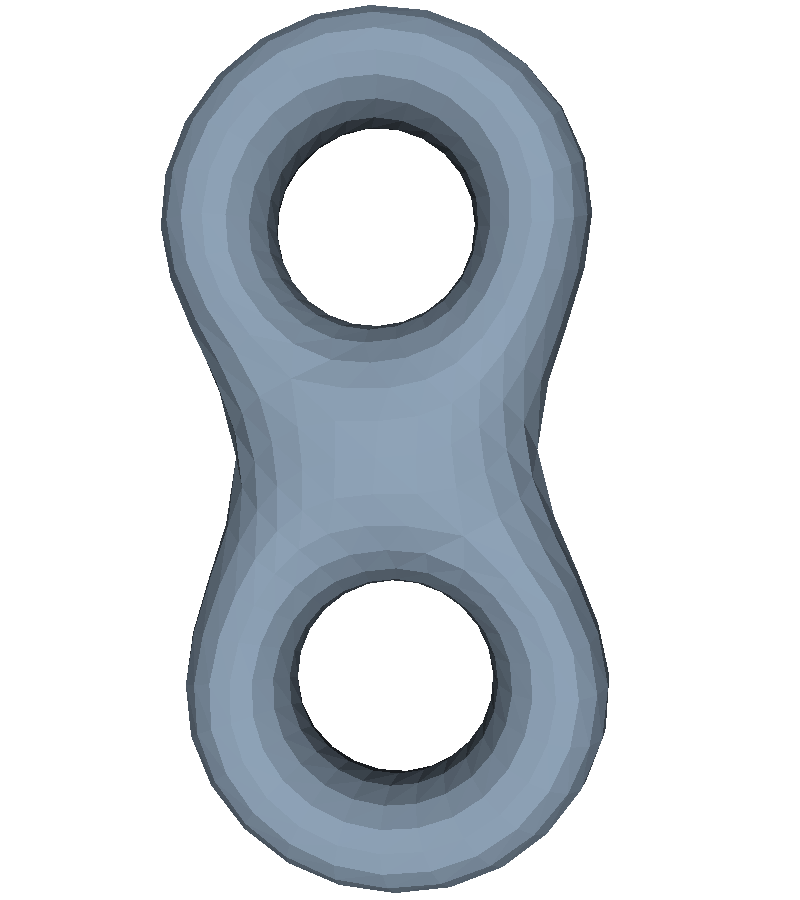
\includegraphics[width=\linewidth]{FIG1}
        \caption{} \label{fig:eight}
    \end{subfigure}%
    ~
    \begin{subfigure}[b]{0.35\linewidth}
        \includegraphics[width=\linewidth]{FIG2}
        \caption{} \label{fig:eight:coord}
    \end{subfigure}
    ~
    \begin{subfigure}[b]{0.35\linewidth}
        \includegraphics[width=\linewidth]{FIG3}
        \caption{} \label{fig:eight:spectral:coeff}
    \end{subfigure}%
    \\
    \begin{subfigure}[b]{0.4\linewidth}
        \includegraphics[width=\linewidth]{FIG4}
        \caption{} \label{fig:eight:spectral:energy}
    \end{subfigure}
    ~
    \begin{subfigure}[b]{0.4\linewidth}
        \includegraphics[width=\linewidth]{FIG5}
        \caption{} \label{fig:eight:spectral:approx:error}
    \end{subfigure}
    \caption[Approximation of the double-torus model with Laplacian eigenbasis.]
      {Approximation of the double-torus model with the Laplacian
      eigenbasis. (a) Original shape; (b) Vertex coordinate functions;
      (c) Spectral coefficients of the coordinate functions w.r.t. the
      Laplacian eigenbasis; (d) Ratios of spectral energy contained in
      the first $k$ coefficients; (e) Approximation error of the mesh
      geometry using the first $k$ coefficients.}
\label{fig:spectral}
\end{figure}

As an example, Fig.~\ref{fig:spectral} shows the power of Laplacian
eigenbasis for shape approximation. Fig.~\ref{fig:spectral}(b)-(c)
visualize the mesh coordinate functions of the example mesh and their
spectral transform coefficients, respectively. We can easily see that
the coordinate functions have very dense support in the natural graph
basis, but can be sparsely represented in the spectral/Fourier domain
in the sense that the majority of spectral coefficients are almost 0.
Moreover, the few significant coefficients are mostly concentrated in
the low-frequency end, especially for a smooth shape model.

Fig.~\ref{fig:spectral}(d) shows the spectral energies contained in
the first $k$ coefficients (linear approximation) and the first $k$
most significant coefficients (nonlinear approximation). We see that
the vast majority of spectral energy are captured by the first few
significant coefficients.

Fig.~\ref{fig:spectral}(e) shows how the mesh reconstruction error
changes with the number of coefficients being used. In this example,
we see that the approximation error becomes negligible using only
about 20 non-zero coefficients.

\subsection{Surface Inpainting}

In the previous section, we have shown that the geometry of a 3D shape
generally has a sparse representation w.r.t. its Laplacian
eigenbasis. Hence, we can set the Laplacian eigenvector as the
reconstruction dictionary and use the sparsity of coefficients as a
prior to estimate the representation of missing shape geometry.

Following the formulation in Sec.~\ref{sec:inpaint:model}, surface inpainting
can be rewritten as the following sparse approximation problem
\begin{equation}
\label{eq:sa}
\hat{\mathbf{\alpha}} = \arg\min_{\mathbf{\alpha}} \|\mathbf{\alpha}\|_0 \quad \text{s.t.} \quad \|P\Phi\mathbf{\alpha} - \mathbf{x}'\|_2^2 < \epsilon,
\end{equation}
\begin{equation}
\hat{\mathbf{x}} = \Phi \mathbf{\alpha}.
\end{equation}
Here the pseudo-norm $\|\mathbf{\alpha}\|_0 = \#\{ i : \alpha_i \neq
0\}$ denotes the support of $\mathbf{\alpha}$, which counts the number
of non-zero components of $\mathbf{\alpha}$, $\Phi$ denotes the
dictionary matrix comprising the Laplacian eigenfunctions, and
$\hat{\mathbf{x}}$ and $\mathbf{x}'$ represent the estimated and
observable coordinate functions, respectively.

We should note that, since the Laplacian eigenbasis constitute a
complete dictionary, Eq.~\ref{eq:sa} is solvable even if we set
$\epsilon=0$, in which case the reconstructed shape will exactly
match the known geometry. However, strictly sparse signals are rare in
real life. It is much more likely that the unknown shape geometry is
\emph{compressible} or \emph{weakly sparse} w.r.t. the dictionary of
Laplacian eigenvectors, i.e., the nonlinear approximation
errors observe a power law decay as the number of participating basis vectors
increases~\cite{Starck2010}. In practice, we set $\epsilon > 0$ to
trade off exact reproduction for a sparser $\alpha$, i.e., allowing the
reconstructed signal to have small discrepancies with the observation.

Solving $l_0$ optimization is an NP-hard problem in nature.
Fortunately, under certain conditions, greedy algorithms such as
orthogonal matching pursuit (OMP) and its variants can generate the
exact sparse solution or a good enough
approximation~\cite{Needell2010,Tropp2007}.

Another approach to find an approximated solution to Eq.~\ref{eq:sa}
is to relax the highly discontinuous $l_0$ norm with $l_1$ norm, i.e.
\begin{equation}
\label{eq:bpdn}
\hat{\mathbf{\alpha}} = \arg\min_{\mathbf{\alpha}} \|\mathbf{\alpha}\|_1 \quad \text{s.t.} \quad \|P\Phi\mathbf{\alpha} - \mathbf{x}'\|_2^2 < \epsilon,
\end{equation}
or equivalently,
\begin{equation}
\label{eq:bpdn2}
\hat{\mathbf{\alpha}} = \arg\min_{\mathbf{\alpha}} \|P\Phi\mathbf{\alpha} - \mathbf{x}'\|_2^2 + \lambda\|\mathbf{\alpha}\|_1.
\end{equation}

The estimation problem then becomes convex and solvable. There are
several readily available algorithms for solving $l_1$ optimization,
e.g., interior point method~\cite{Kim2007}, iteratively reweighted
least squares (IRLS)~\cite{Holland1977}, least angle regression
(LARS)~\cite{Sorkine2004}, and iterative
shrinkage-thresholding~\cite{Daubechies2004}.

For the task of surface inpainting, we find that $l_1$ optimization algorithms tend to be
more robust and generally produce better inpainting results than greedy algorithms. In this work,
we use the l1\_ls solver introduced in \cite{Kim2007} which implements a fast interior-point method
for solving $l_1$-regularized least-square problems like Eq.~\ref{eq:bpdn2}.

\begin{figure}
    \centering
    \begin{subfigure}[b]{0.36\linewidth}
        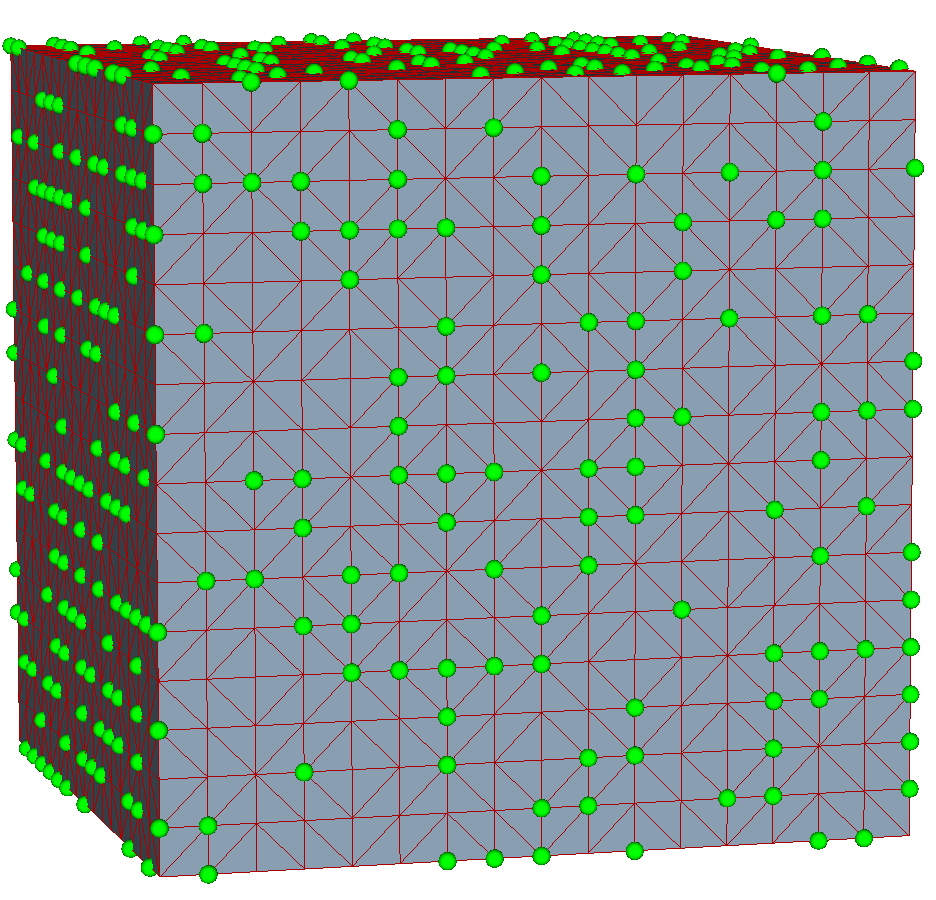
\includegraphics[width=\linewidth]{FIG6}
        \caption{}
    \end{subfigure}%
    ~
    \begin{subfigure}[b]{0.36\linewidth}
        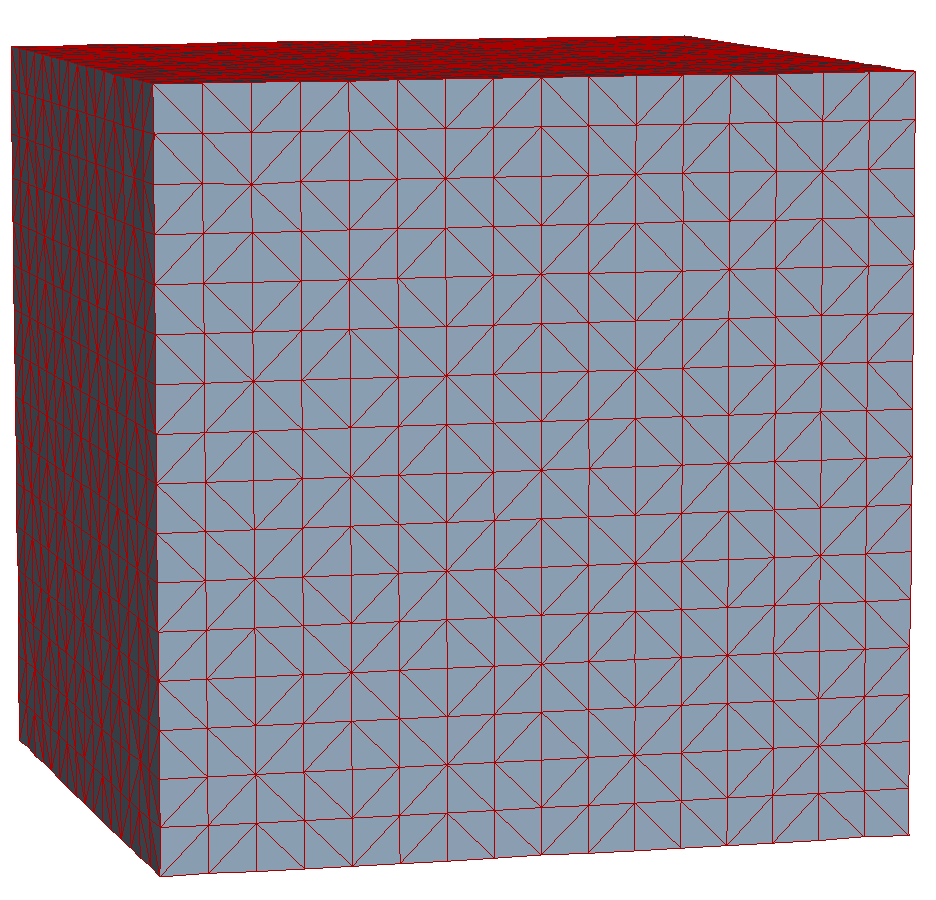
\includegraphics[width=\linewidth]{FIG7}
        \caption{}
    \end{subfigure}%
    \\
    \begin{subfigure}[b]{0.4\linewidth}
        \includegraphics[width=\linewidth]{FIG8}
        \caption{}
    \end{subfigure}%
    ~
    \begin{subfigure}[b]{0.4\linewidth}
        \includegraphics[width=\linewidth]{FIG9}
        \caption{}
    \end{subfigure}%
    \caption[Estimating Laplacian eigenbasis coefficients with partial cube model.]
      {Estimating the Laplacian eigenbasis coefficients of the
      cube model with 40\% random missing vertices. (a) Original shape model;
      green dots denote vertices that are labelled as missing. (b) The
      reconstructed shape using our inpainting method. (c) The
      coefficient representation of the original shape's
      x-coordinates. (d) Estimated coefficient representation of the
      x-coordinates inferred from the information of available
      vertices. }
\label{fig:cube:random:inpaint}
\end{figure}

As an example, Fig.~\ref{fig:cube:random:inpaint} demonstrates the
potentials of our sparsity-based inpainting method. We randomly label
40\% of vertices of the original cube model as missing vertices, and
use the coordinates of the remaining vertices to estimate the spectral
coefficient representation of the original shape by solving
Eq.~\ref{eq:bpdn}. Fig.~\ref{fig:cube:random:inpaint}(b) shows the
shape reconstructed from the estimated spectral coefficients.
Fig.~\ref{fig:cube:random:inpaint}(c)-(d) shows the spectral
coefficients computed from the original x-coordinate function and the
coefficients estimated by our sparsity-based method, respectively. In
this example, our method recovers the sparse coefficient
representation in a very precise way.


\subsection{Filling Surface Holes}
\label{sec:inpaint:holefilling}

One of the most important technical elements of our surface inpainting
method is the dictionary of global shape basis, which are determined by
the global mesh connectivity. For some applications such as repairing
damaged surface regions, the mesh connectivity of the region to be
repaired is already known in advance before reconstruction and we may
not need to modify it. For hole filling applications, however, the
inpainting regions are completely blank without any inside
information. It is imperative to establish interior mesh connectivity,
by way of vertex insertion and patch triangulation, before our surface
inpainting method can be applied.

Obviously, how a patch (to be used to cover the hole region) is
triangulated directly influences the final inpainting result in our
framework. In general, a good patch triangulation should ensure the
vertex density of the inserted mesh to be consistent with the
remaining mesh. In this work, we adopt the algorithms proposed by
Liepa in \cite{Liepa2003} for hole triangulation and refinement.
Algorithm~\ref{algo:holefilling} summarizes the pipeline of our
sparsity-based hole filling method.

\begin{algorithm}
\caption{Sparsity-Based Hole Filling}
\label{algo:holefilling}
\begin{algorithmic}[1]
  \REQUIRE Input mesh $M$
\STATE Identify surface holes,
\STATE Triangulate and refine holes using the algorithms described in
  \cite{Liepa2003},
\STATE Compute the mesh Laplace matrix $L$ and the Laplacian eigenbasis dictionary $\Phi$,
\FOR{coordinate $\mathbf{x}$, $\mathbf{y}$, and $\mathbf{z}$}
\STATE Compute the spectral representation $\mathbf{\alpha}$ of the global coordinates by solving Eq.~\ref{eq:bpdn},
\STATE Reconstruct the coordinates of the inserted mesh with $\Phi\mathbf{\alpha}$,
\ENDFOR
\end{algorithmic}
\end{algorithm}

\subsection{Remarks on Dictionary}
\label{sec:inpaint:remark}

Although the dictionary of Laplacian eigenvectors in general has strong
compressive power for encoding shape geometry, it also has some limitations.
Similar to Fourier basis, the Laplacian eigenvectors are most suitable for
representing smooth signals or globally repetitive features, but are generally
not optimized for encoding shapes with many local sharp features. In the image
domain, other than 2D Fourier basis, people have developed various types of
harmonic basis (e.g., wavelet, curvelet, ridgelet, etc) for efficient encoding
of images of different properties. For example, the ridgelets are especially
efficient in representing piecewise smooth images with global straight
edges~\cite{Fadili2012}. In the mesh domain, however, we do not have such
diverse harmonic basis to choose from, which for now limits the power of
sparsity-based methods.

Another issue is related to the ratio of Laplacian eigen-decomposition.
Computing the full set of Laplacian eigenvectors of a large mesh is
extremely time consuming, generally infeasible for meshes with more than a few
thousand vertices on a regular PC. Fortunately, for our surface inpainting
applications, it is actually not necessary or even desirable to compute the
full set of eigenvectors. On the one hand, for smooth shapes, the spectral
energy is overwhelmingly concentrated on the low-frequency end, and a
dictionary composed of only low-frequency eigenvectors can well approximate the
shape geometry with very little error. On the other hand, the high-frequency
Laplacian eigenvectors are less stable than the low-frequency ones, and
including them in the dictionary may cause overfitting and result in worse
inpainting results, since the high-frequency eigenvectors are more correlated
with local geometric details than with the overall structure of the shape. In
our experiments, we find that the best inpainting results are usually achieved
with a dictionary of 20\% to 50\% total eigenvectors.


\section{Experiments}
In this section, we first evaluate the performance of our sparsity-based
inpainting algorithms on recovering missing geometry from partial observations.
Then we demonstrate how our method can be applied to repairing damaged geometry
and filling surface holes.

\subsection{Geometry Recovery}
To evaluate the performance of geometry recovery, for each testing model, we
randomly label 20\%-50\% vertices as missing and use our sparsity-based
inpainting method to estimate the original geometry based on the coordinates of
the still available vertices. The estimated coordinates are then compared with
the original coordinates.

All the testing models have been translated and scaled to be contained inside
the unit cube. The recovery error is measured as the
root-mean-square error (RMSE) of the coordinates of the missing vertices.

\begin{figure}
  \centering
    \begin{subfigure}[b]{0.23\linewidth}
        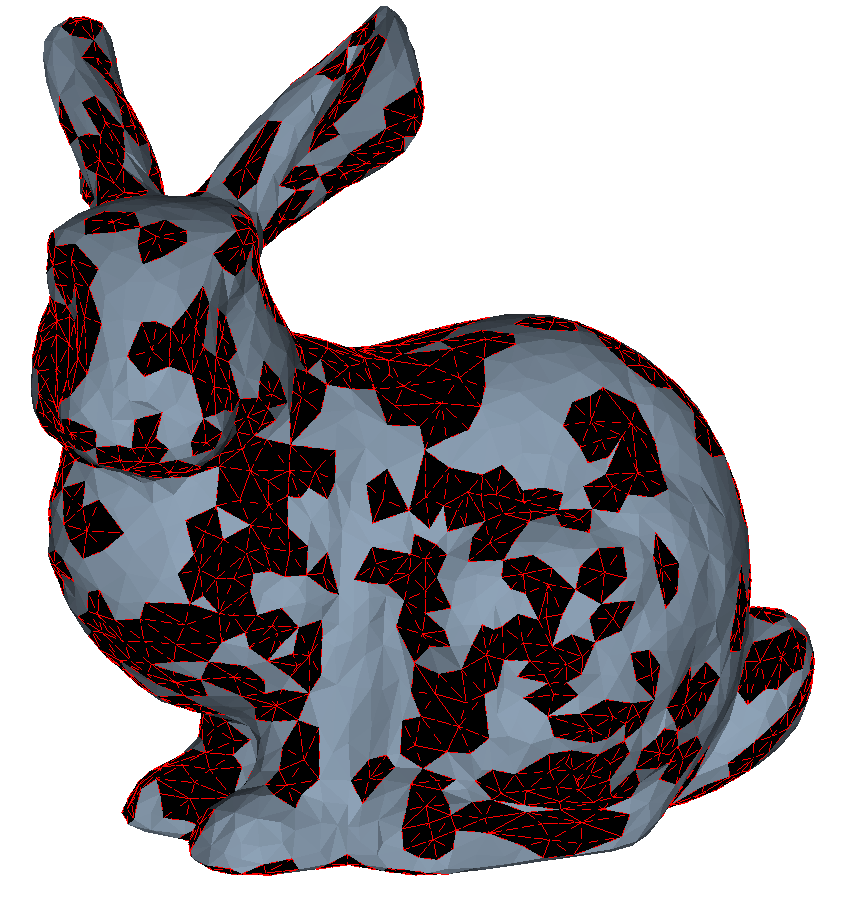
\includegraphics[width=\linewidth]{FIG10}
        \caption{20\% vertices missing.}
    \end{subfigure}
    ~
    \begin{subfigure}[b]{0.23\linewidth}
        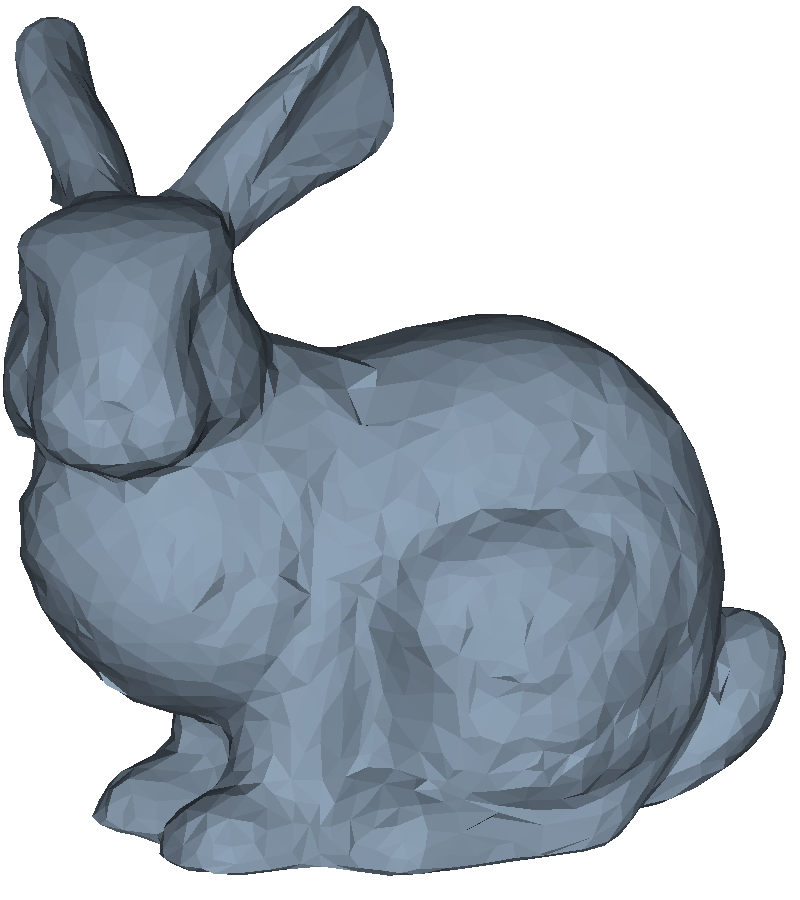
\includegraphics[width=\linewidth]{FIG11}
        \caption{Shape recovered from (a).}
    \end{subfigure}
    ~
    \begin{subfigure}[b]{0.23\linewidth}
        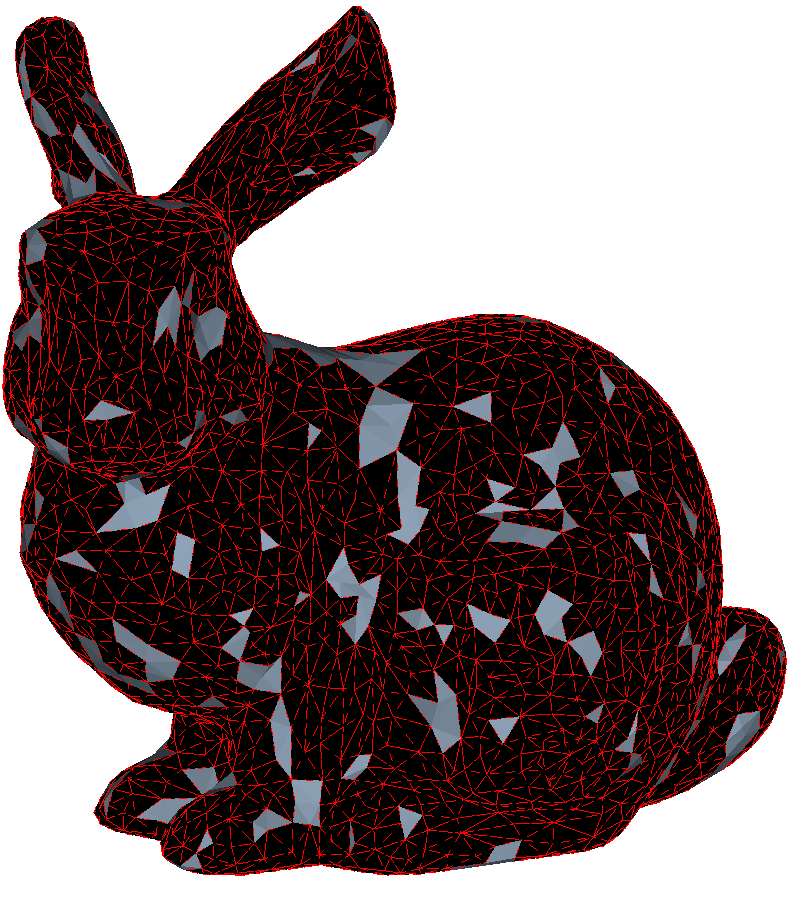
\includegraphics[width=\linewidth]{FIG12}
        \caption{50\% vertices missing.}
    \end{subfigure}
    ~
    \begin{subfigure}[b]{0.23\linewidth}
        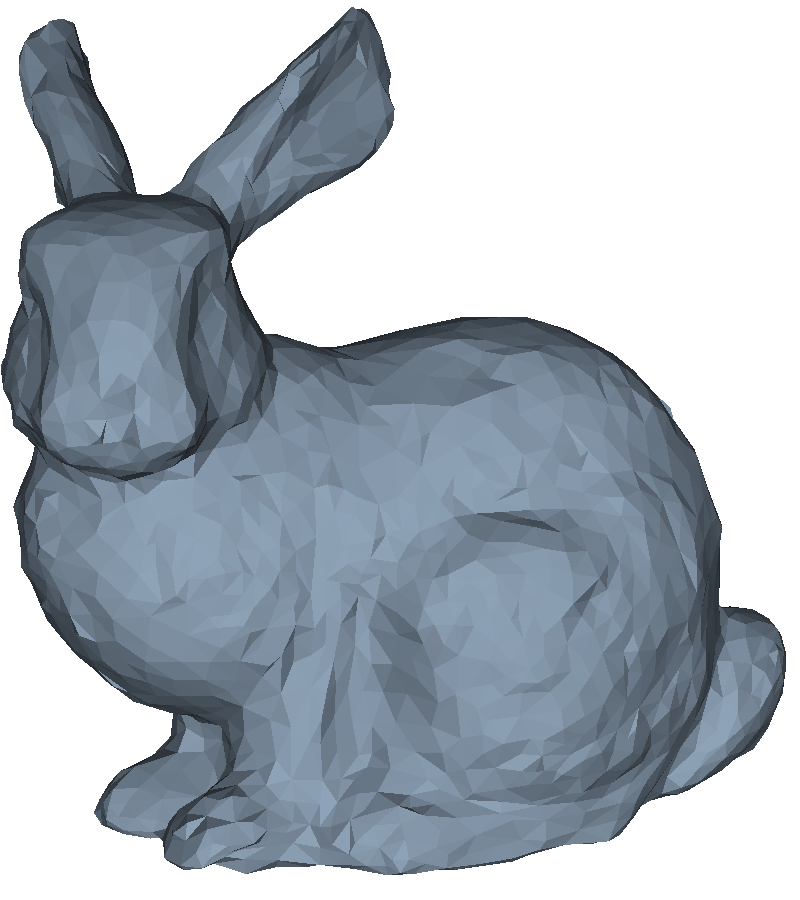
\includegraphics[width=\linewidth]{FIG13}
        \caption{Shape recovered from (c).}
    \end{subfigure}
\caption[Recovery of the bunny model with random missing vertices.]
{Recovery of the bunny model with 20\% and 50\% random missing vertices.}
\label{fig:bunny:recovery}
\end{figure}

\begin{figure}
  \centering
    \begin{subfigure}[b]{0.35\linewidth}
        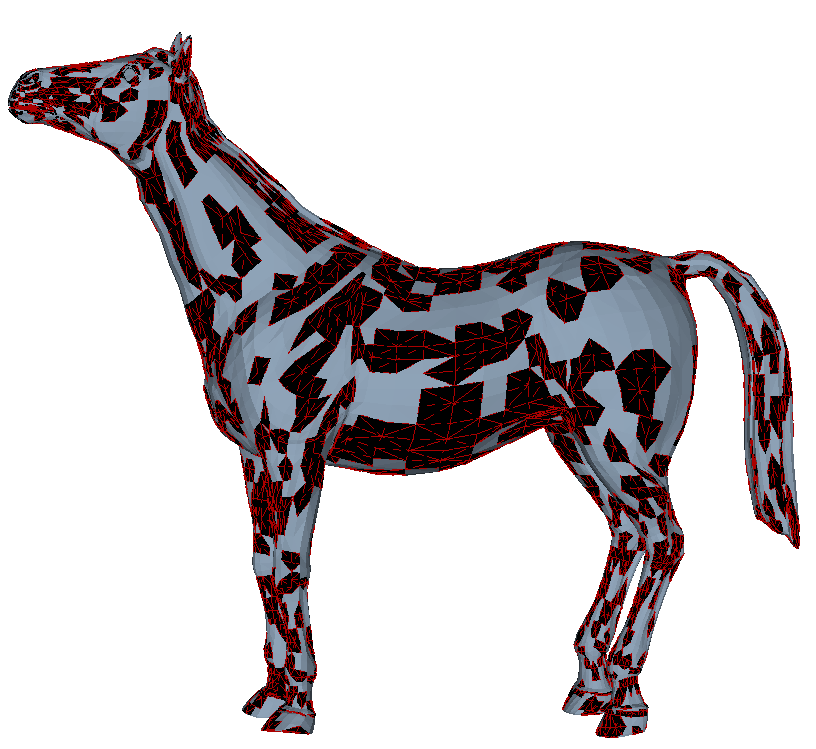
\includegraphics[width=\linewidth]{FIG14}
        \caption{20\% vertices missing.}
    \end{subfigure}
    ~
    \begin{subfigure}[b]{0.35\linewidth}
        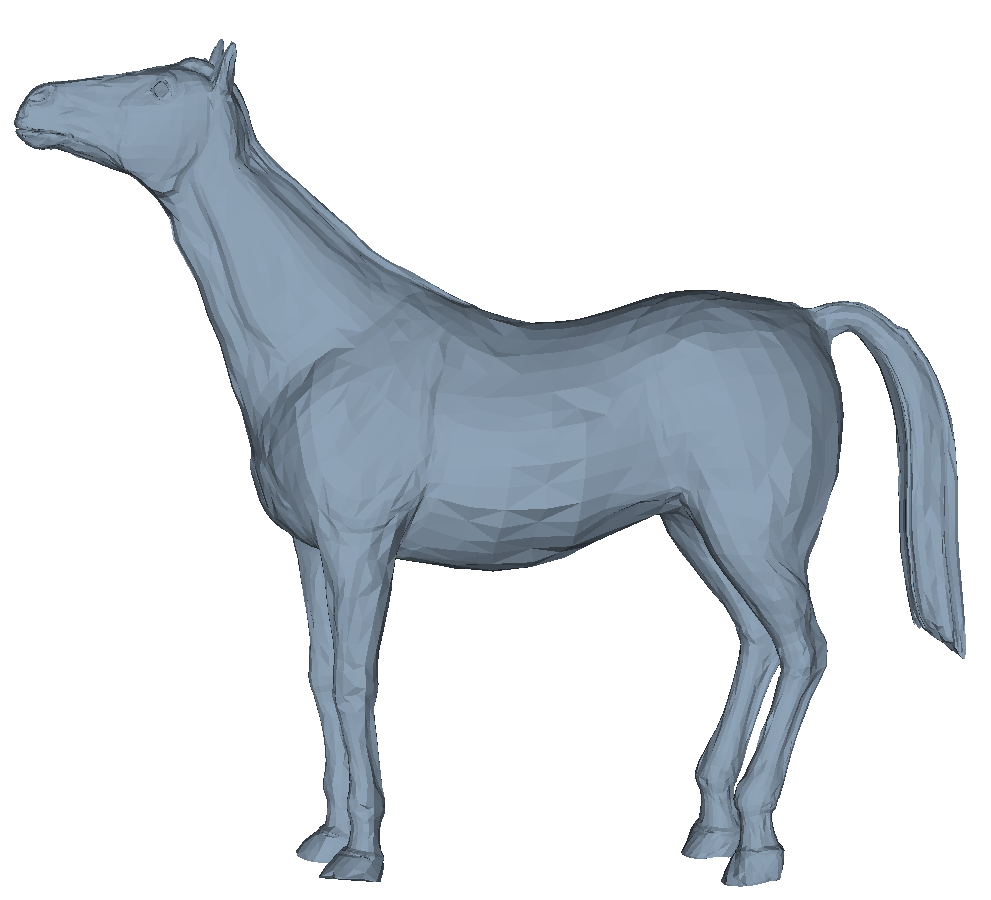
\includegraphics[width=\linewidth]{FIG15}
        \caption{Shape recovered from (a).}
    \end{subfigure}
    \\
    \begin{subfigure}[b]{0.35\linewidth}
        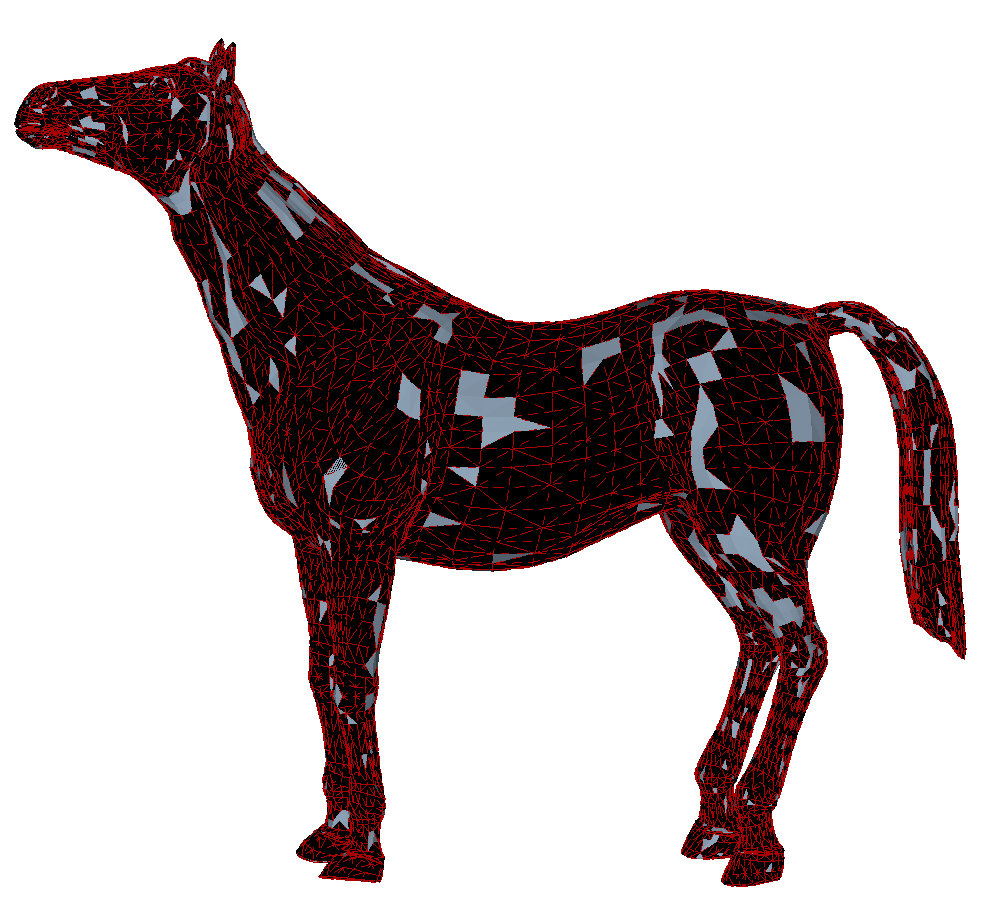
\includegraphics[width=\linewidth]{FIG16}
        \caption{50\% vertices missing.}
    \end{subfigure}
    ~
    \begin{subfigure}[b]{0.35\linewidth}
        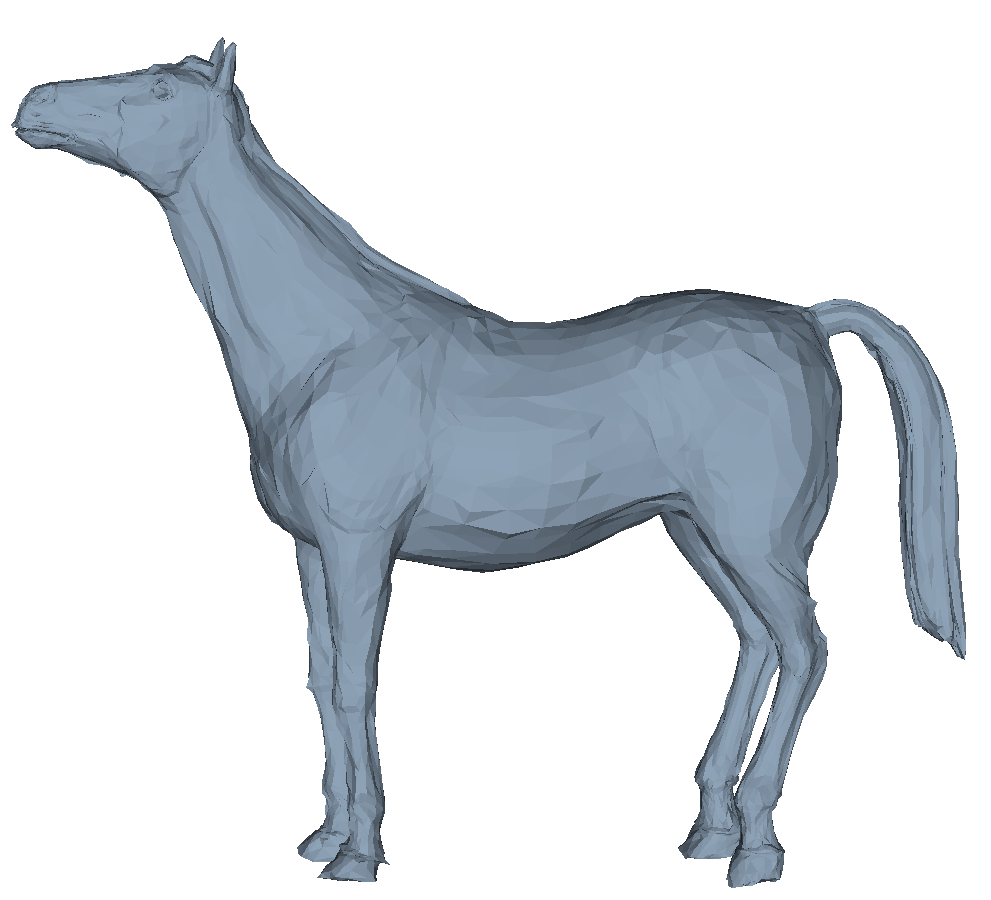
\includegraphics[width=\linewidth]{FIG17}
        \caption{Shape recovered from (c).}
    \end{subfigure}
\caption[Recovery of the horse model with random missing vertices.]
{Recovery of the horse model with 20\% and 50\% random missing vertices.}
\label{fig:horse:recovery}
\end{figure}

\begin{figure}
  \centering
    \begin{subfigure}[b]{0.35\linewidth}
        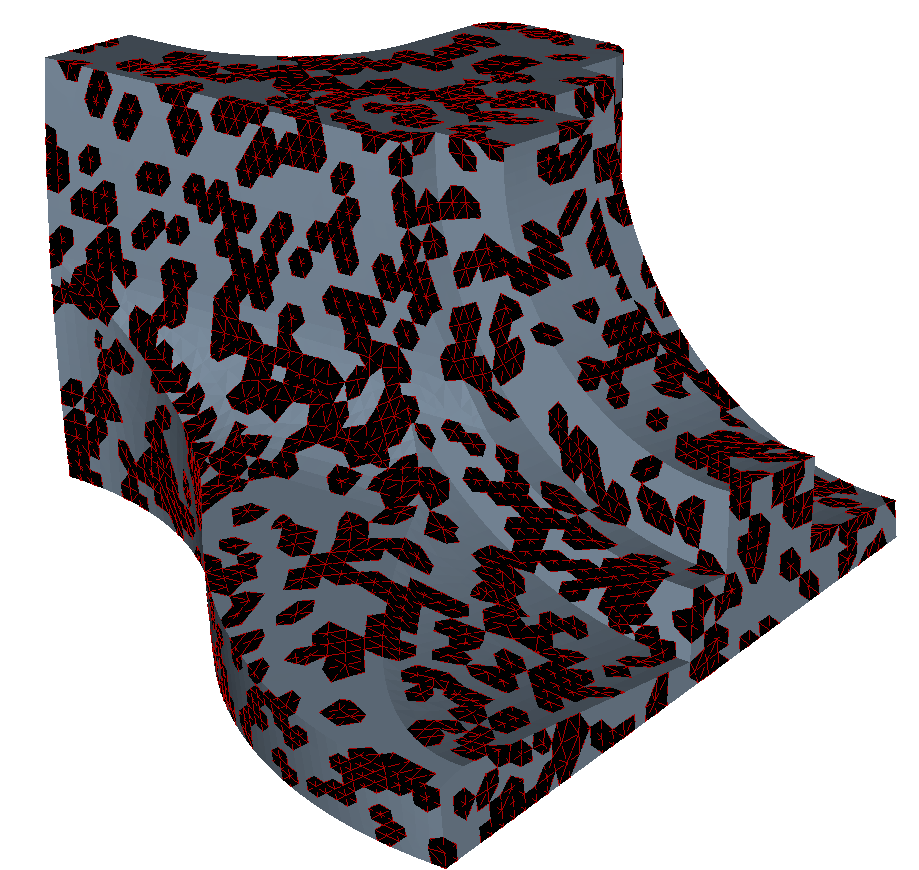
\includegraphics[width=\linewidth]{FIG18}
        \caption{20\% vertices missing.}
    \end{subfigure}
    ~
    \begin{subfigure}[b]{0.35\linewidth}
        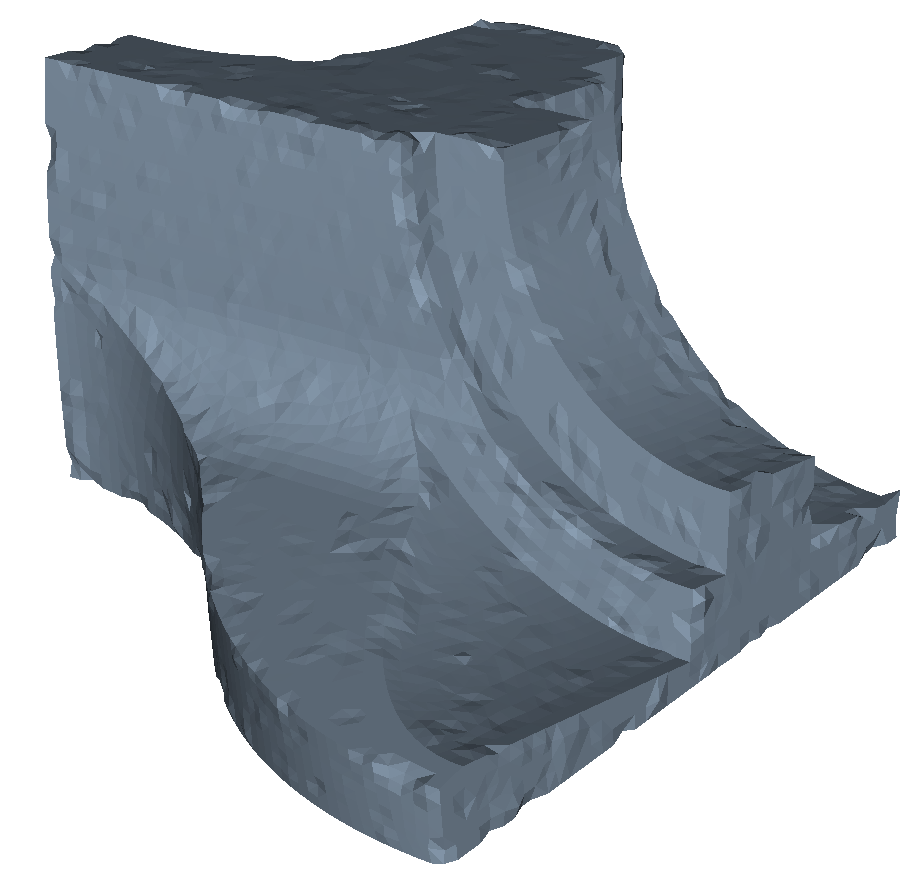
\includegraphics[width=\linewidth]{FIG19}
        \caption{Shape recovered from (a).}
    \end{subfigure}
    \\
    \begin{subfigure}[b]{0.35\linewidth}
        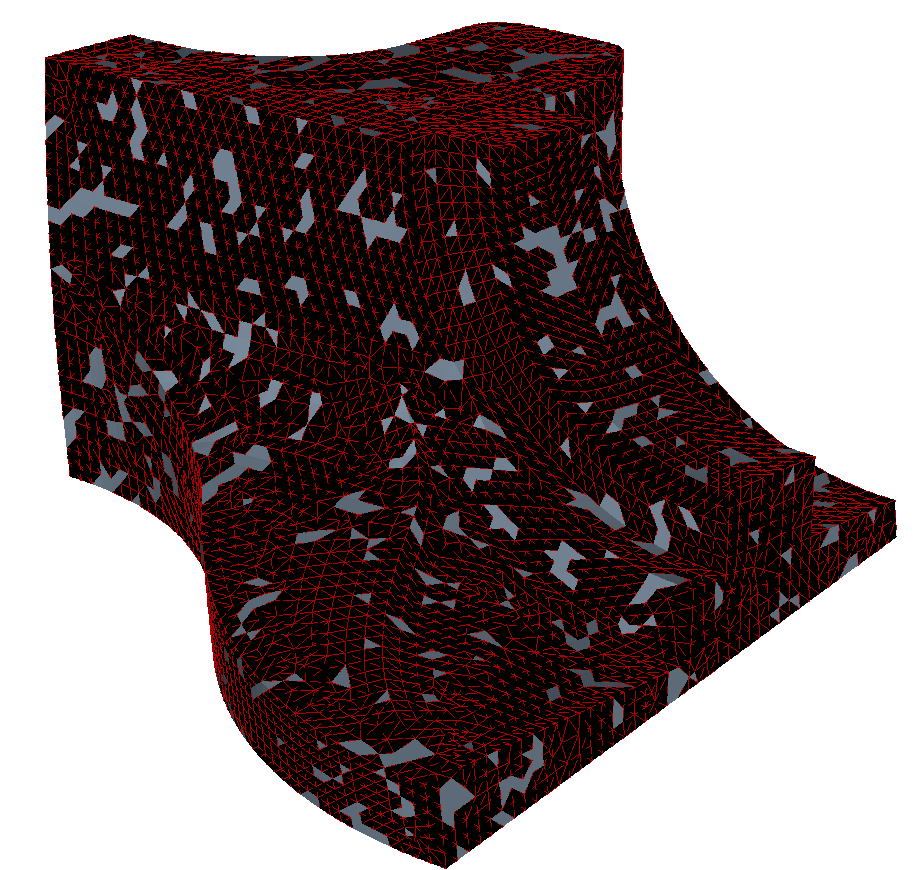
\includegraphics[width=\linewidth]{FIG20}
        \caption{50\% vertices missing.}
    \end{subfigure}
    ~
    \begin{subfigure}[b]{0.35\linewidth}
        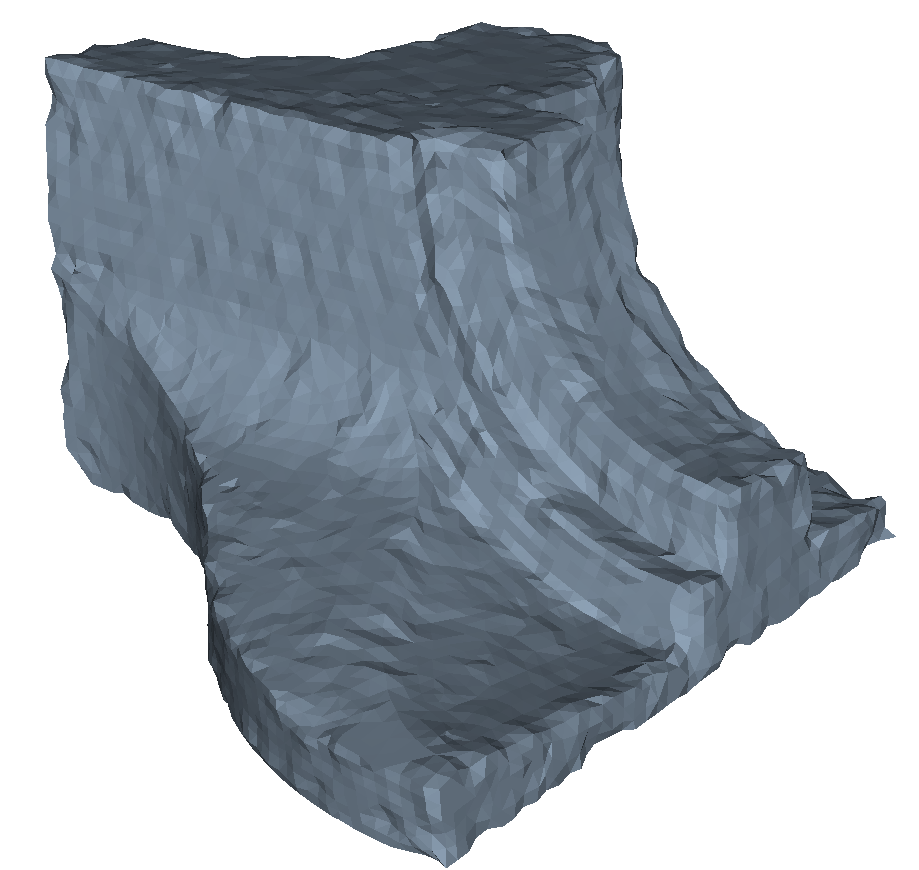
\includegraphics[width=\linewidth]{FIG21}
        \caption{Shape recovered from (c).}
    \end{subfigure}
\caption[Recovery of the fandisk model with random missing vertices.]
{Recovery of the fandisk model with 20\% and 50\% random missing vertices.}
\label{fig:fandisk:recovery}
\end{figure}

\begin{figure}
  \centering
    \begin{subfigure}[b]{0.35\linewidth}
        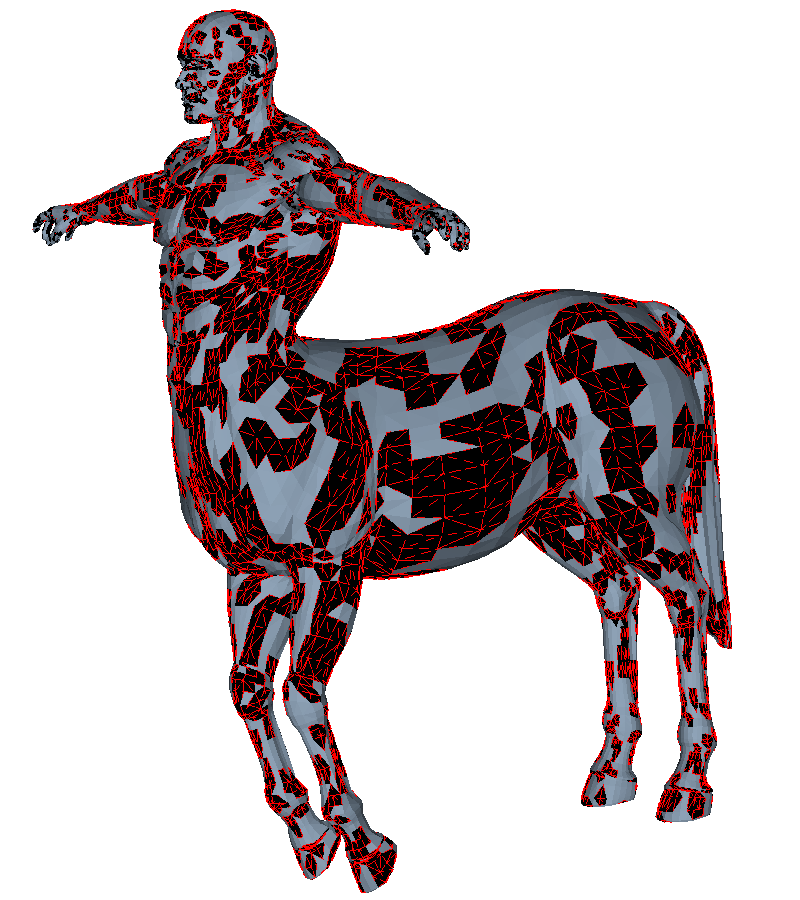
\includegraphics[width=\linewidth]{FIG22}
        \caption{20\% vertices missing.}
    \end{subfigure}
    ~
    \begin{subfigure}[b]{0.35\linewidth}
        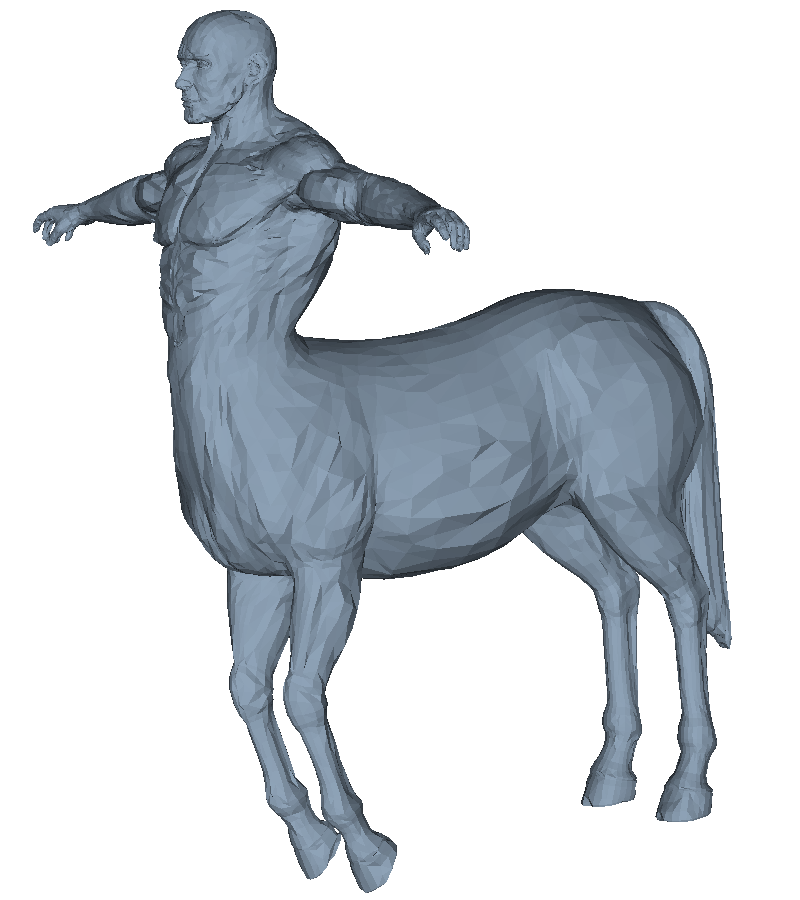
\includegraphics[width=\linewidth]{FIG23}
        \caption{Shape recovered from (a).}
    \end{subfigure}
    \\
    \begin{subfigure}[b]{0.35\linewidth}
        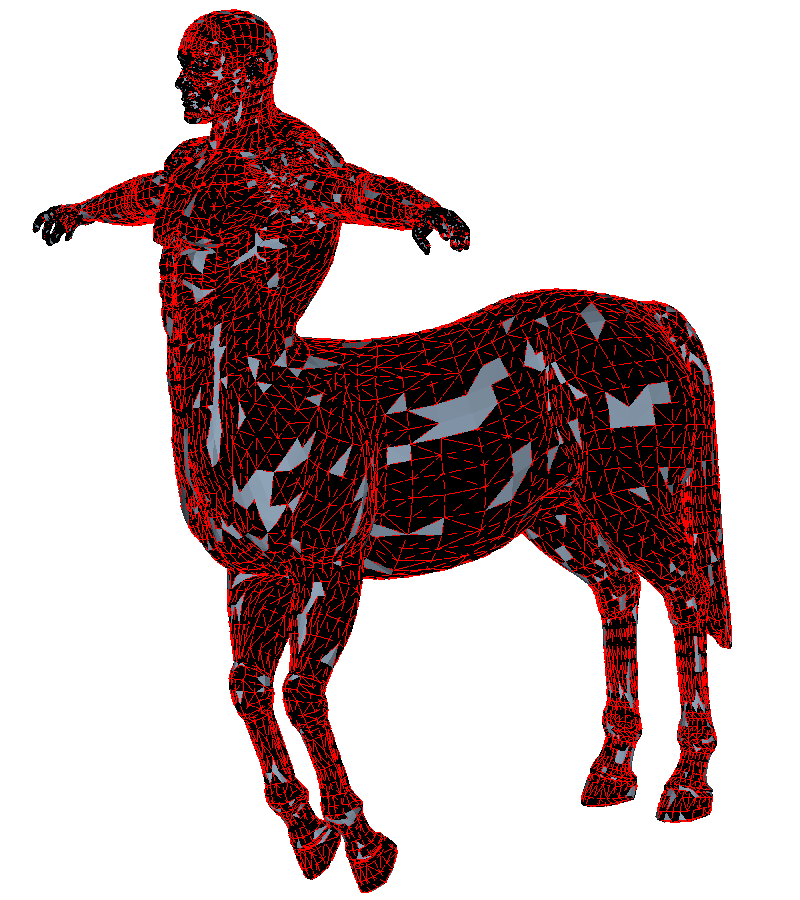
\includegraphics[width=\linewidth]{FIG24}
        \caption{50\% vertices missing.}
    \end{subfigure}
    ~
    \begin{subfigure}[b]{0.35\linewidth}
        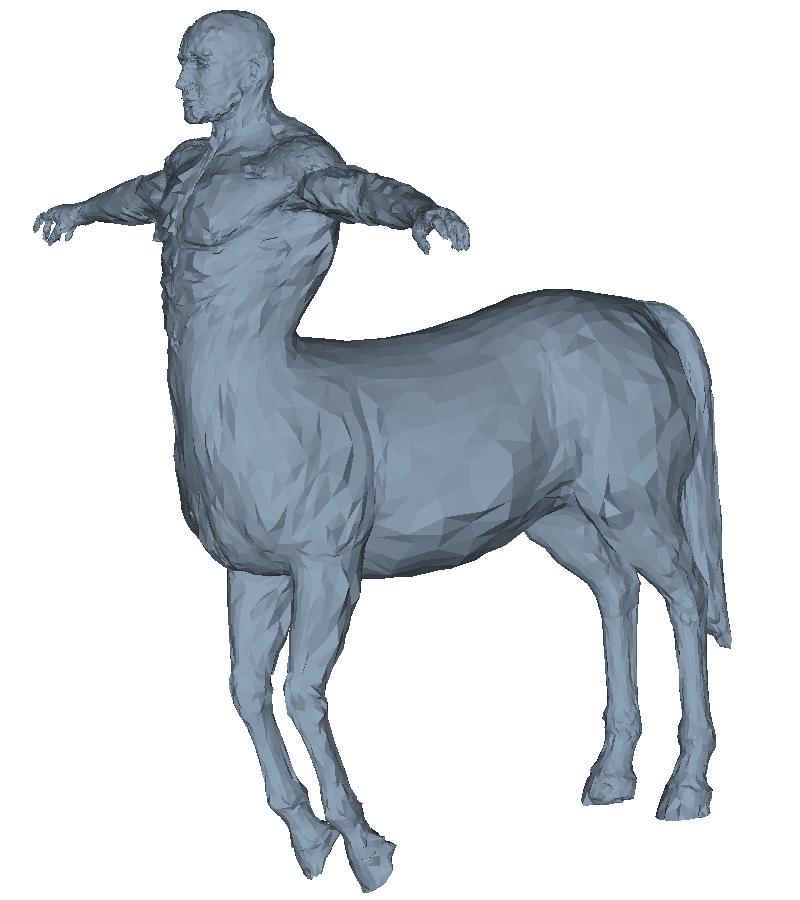
\includegraphics[width=\linewidth]{FIG25}
        \caption{Shape recovered from (c).}
    \end{subfigure}
\caption[Recovery of the centaur model with random missing vertices.]
{Recovery of the centaur model with 20\% and 50\% random missing vertices.}
\label{fig:centaur:recovery}
\end{figure}

\begin{table}
\centering
  \begin{tabular}{|c|c|c|c|c|c|c|}
  \hline
  Mesh                     & \#vertices                 & \#eigenvectors          & \pbox{20cm}{Decomposition\\ time (s)}        & \pbox{15cm}{Missing\\ ratio} & Error  & $l_1$ time (s) \\
  \hline
  \multirow{2}{3em}{bunny} & \multirow{2}{4em}{2.5k}    & \multirow{2}{5em}{1000} & \multirow{2}{5em}{19.6}   & 0.2          & 1.9e-2 & 2.8       \\
                           &                            &                         &                           & 0.5           & 2.2e-2 & 2.1       \\

  \hline
  \multirow{2}{3em}{horse} & \multirow{2}{4em}{8.4k}    & \multirow{2}{5em}{4000} & \multirow{2}{5em}{1015.4} & 0.2          & 8.6e-3 & 19.7      \\
                           &                            &                         &                           & 0.5           & 1.0e-2 & 59.0      \\
  \hline
  \multirow{2}{3em}{fandisk} & \multirow{2}{4em}{6.5k} & \multirow{2}{5em}{3000} & \multirow{2}{5em}{445.2}   & 0.2          & 8.8e-3 & 17.4      \\
                             &                          &                         &                           & 0.5           & 1.2e-2 & 33.9      \\
  \hline
  \multirow{2}{3em}{centaur} & \multirow{2}{4em}{15.8k} & \multirow{2}{5em}{2000} & \multirow{2}{5em}{397.7}  & 0.2          & 7.1e-3 & 12.2      \\
                             &                          &                         &                           & 0.5           & 8.0e-3 & 15.0      \\
  \hline
  \end{tabular}
\caption[Geometry recovery errors and time performance.]
{Geometry recovery errors and time performance. For each model, we test the recovery performance with
20\% and 50\% randomly selected vertices labelled as missing. Each experiment has been repeated three times
and averaged on a system with quad-core 2.4GHz CPU and 16GB RAM. }
\label{tab:recovery}
\end{table}

Fig.~\ref{fig:bunny:recovery}, Fig.~\ref{fig:horse:recovery}, Fig.~\ref{fig:fandisk:recovery}, and Fig.~\ref{fig:centaur:recovery}
show some examples of geometry recovery with 20\% and 50\%  missing vertices. Table~\ref{tab:recovery} documents
the recovery errors and time performance of our tests. From the experimental results, we have the following
observations:

\begin{itemize}
  \item When the missing vertices are randomly dispersed on the shape, our
        sparsity-based method can reliably recover the missing coordinates
        with great precision, even when the ratios of missing vertices are
        as high as 50\%.
  \item The $l_1$ estimation generally becomes more time consuming when the
        ratio of missing vertices increases.
  \item As noted in Sec.~\ref{sec:inpaint:remark}, using the truncated Laplacian
        eigenbasis dictionary is acceptable for restoring smooth shapes.
        However, for shapes with many edges and corners, such as the fandisk
        model (see Fig.~\ref{fig:fandisk:recovery}), our inpainting method
        cannot well preserve local discontinuities, since the high-frequency
        basis are simply not present in the truncated dictionary.
\end{itemize}

\subsection{Geometry Repair}
Our sparsity-based inpainting method is very suitable for repairing partially
damaged geometry. After manually selecting the damaged regions, we can apply
our inpainting method to estimate the original whole shape with the same
connectivity based on the remaining parts of the shape. The corrupted regions
can then be substituted by the inpainting patch.

\begin{figure}
    \centering
    \begin{subfigure}[b]{0.23\linewidth}
        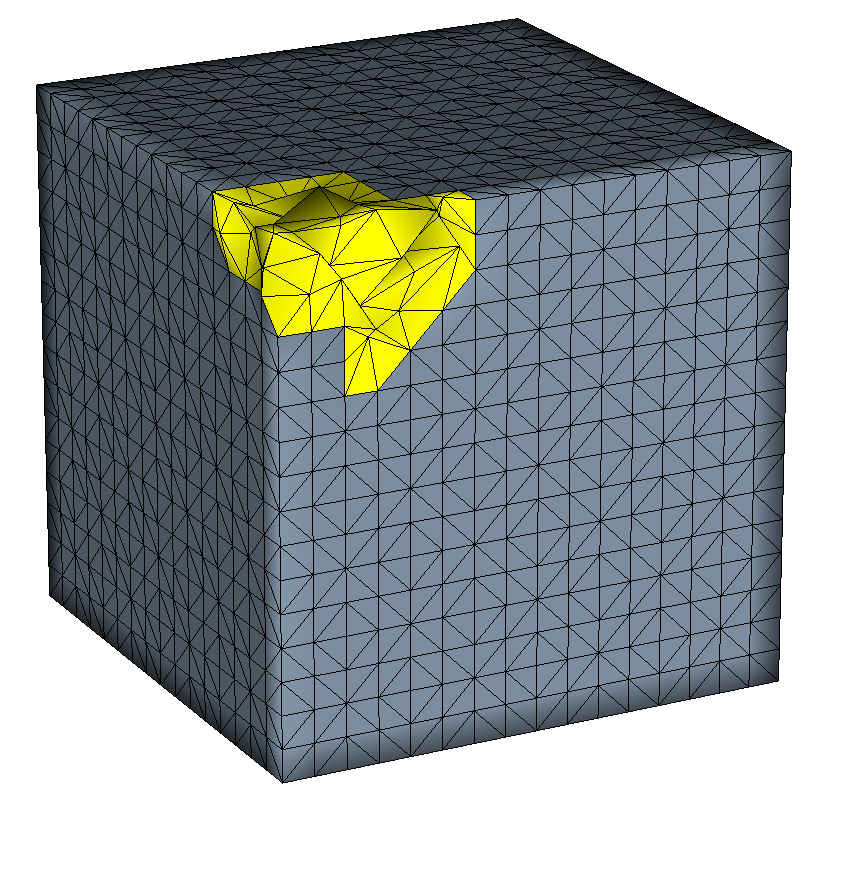
\includegraphics[width=\linewidth]{FIG26}
        \caption{}
    \end{subfigure}%
    ~
    \begin{subfigure}[b]{0.23\linewidth}
        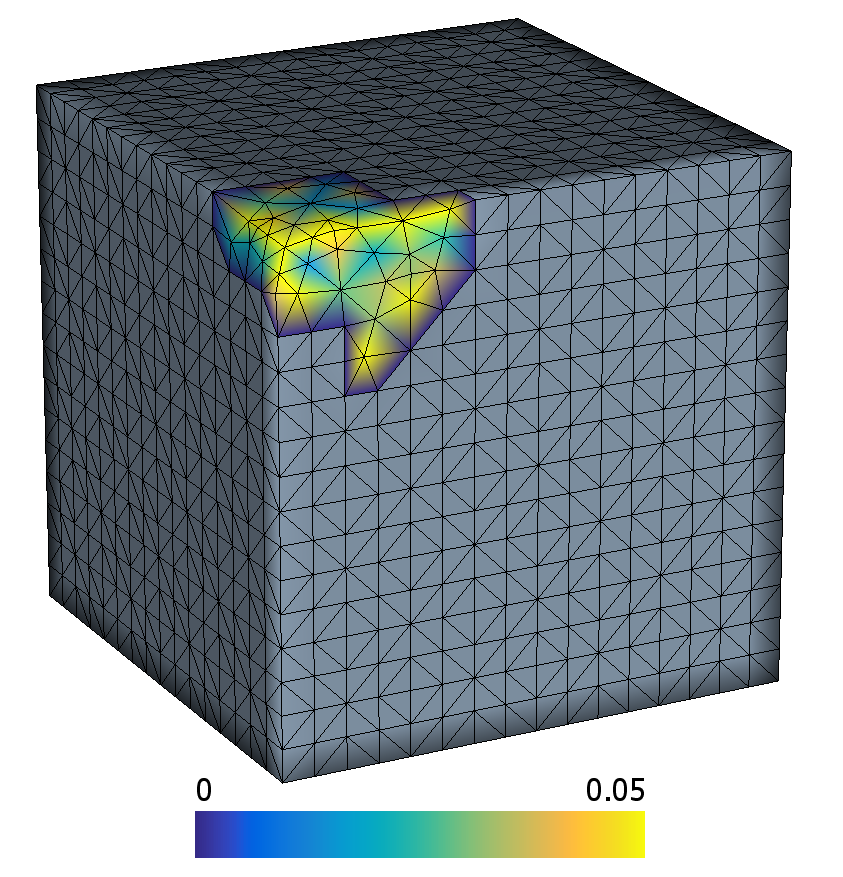
\includegraphics[width=\linewidth]{FIG27}
        \caption{}
    \end{subfigure}
    ~
    \begin{subfigure}[b]{0.23\linewidth}
        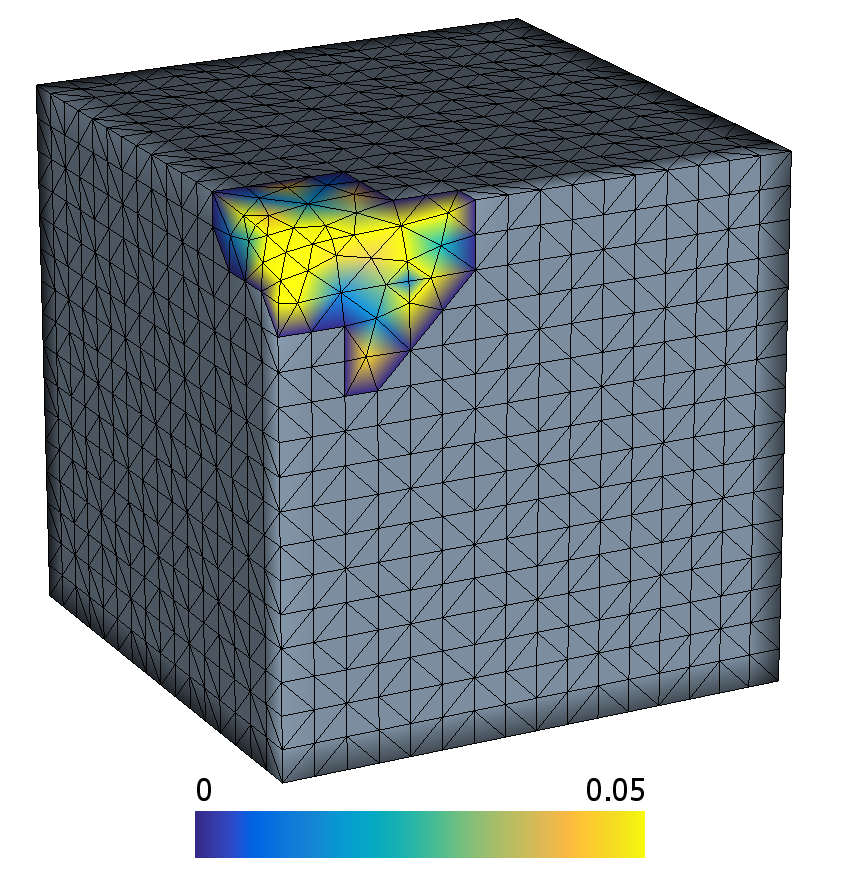
\includegraphics[width=\linewidth]{FIG28}
        \caption{}
    \end{subfigure}
    ~
    \begin{subfigure}[b]{0.23\linewidth}
        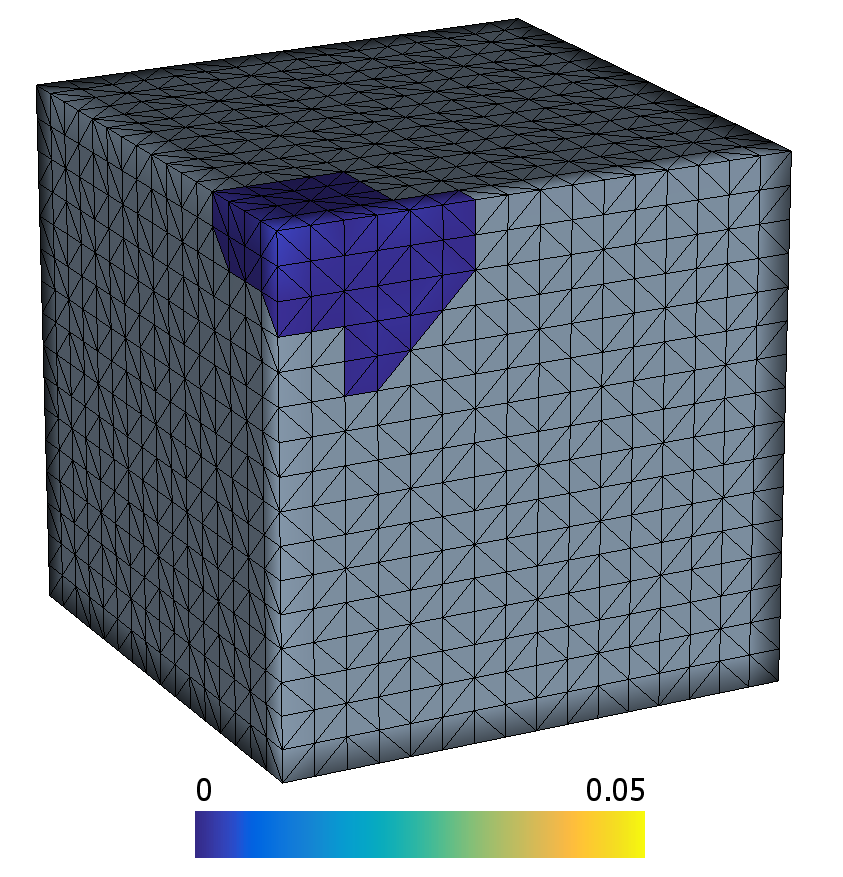
\includegraphics[width=\linewidth]{FIG29}
        \caption{}
    \end{subfigure}
\caption[Geometry repair of the damaged cube model.] 
        {Geometry repair of the cube model by replacing the selected damaged regions (marked in yellow) with an inpainting patch.
         (a) The damaged model; (b) Repaired with Laplacian regularized least square smoothing~\cite{Nealen2006};
         (c) Repaired with thin-plate energy minimization~\cite{Bac2008};
         (d) Repaired with our inpainting method. In (b)-(d), the per-vertex error (compared with the ground truth) is color-coded.}
\label{fig:repair:cube}
\end{figure}

\begin{figure}
    \centering
    \begin{subfigure}[b]{0.23\linewidth}
        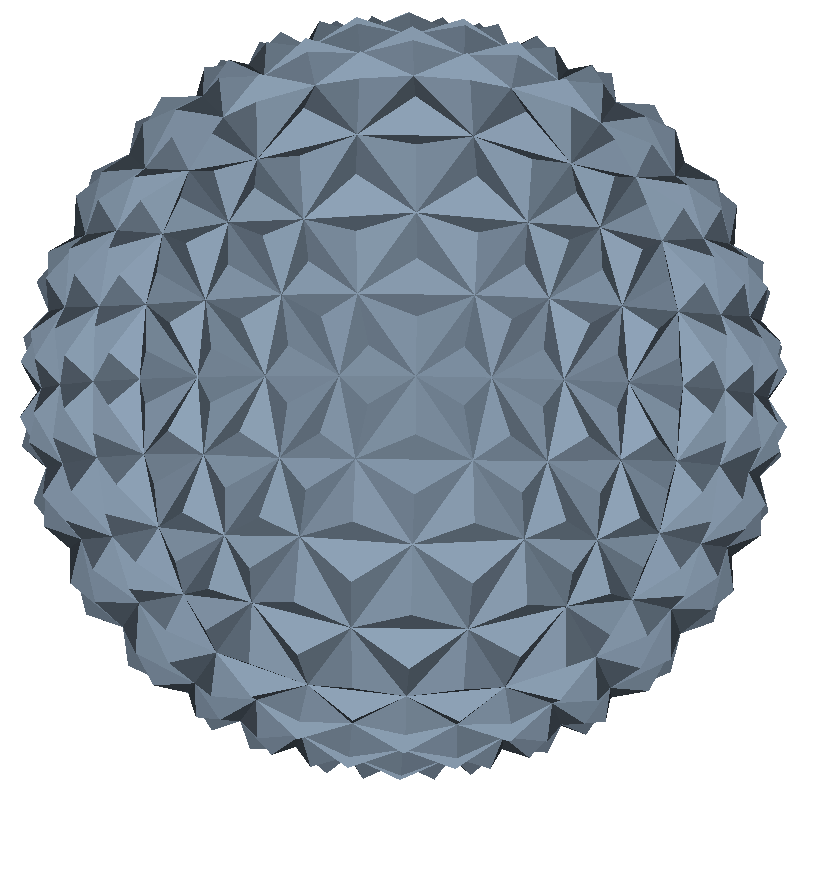
\includegraphics[width=\linewidth]{FIG30}
        \caption{}
    \end{subfigure}%
    ~
    \begin{subfigure}[b]{0.23\linewidth}
        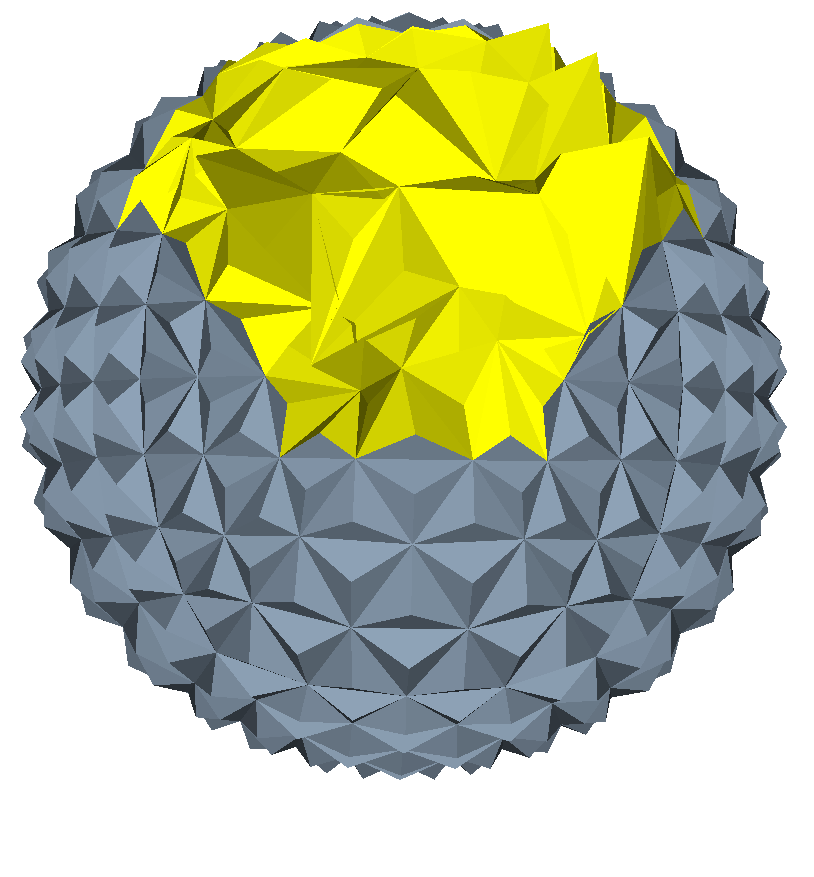
\includegraphics[width=\linewidth]{FIG31}
        \caption{}
    \end{subfigure}
    ~
    \begin{subfigure}[b]{0.23\linewidth}
        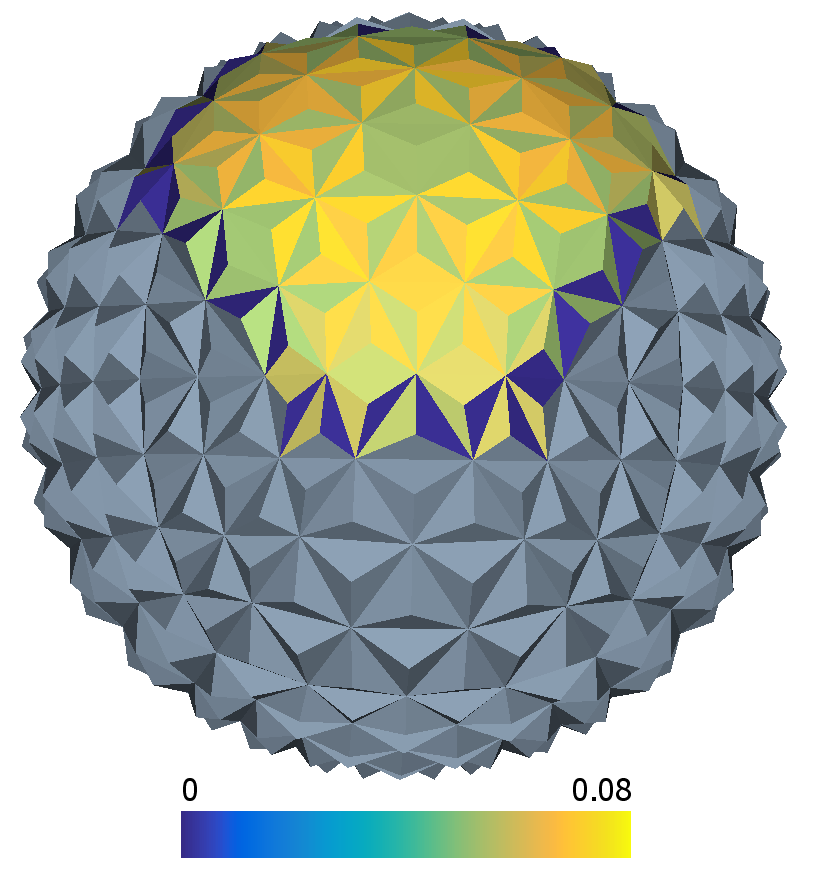
\includegraphics[width=\linewidth]{FIG32}
        \caption{}
    \end{subfigure}
    ~
    \begin{subfigure}[b]{0.23\linewidth}
        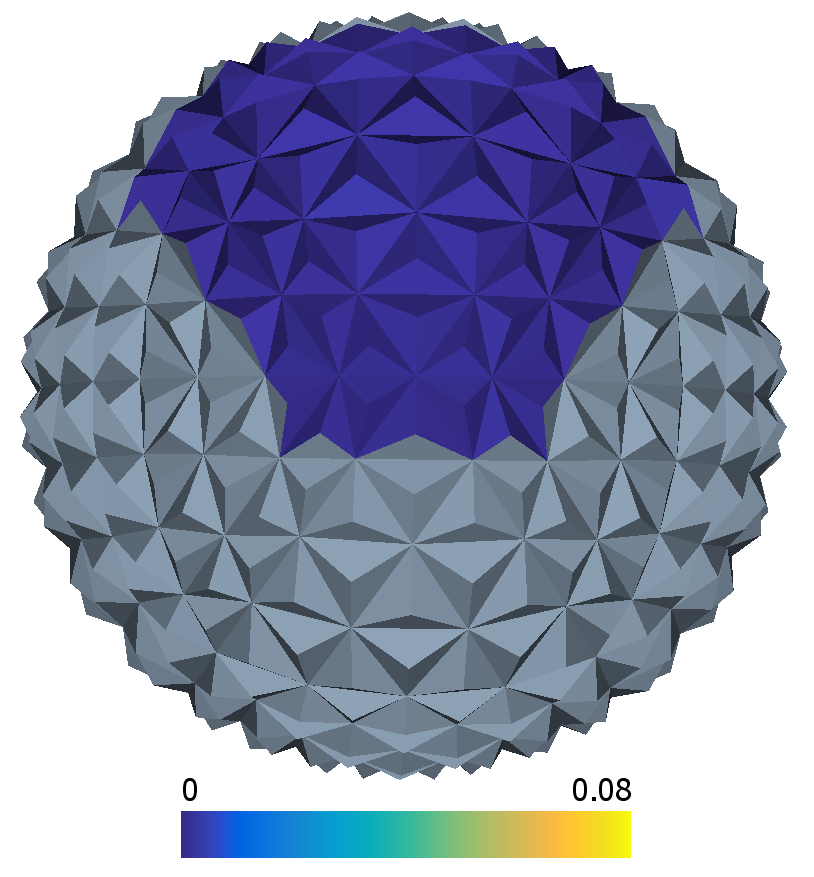
\includegraphics[width=\linewidth]{FIG33}
        \caption{}
    \end{subfigure}
    \caption[Geometry repair of the damaged epcot model.] 
    {Geometry repair of the damaged epcot model. (a) The original epcot model;
    (b) The damaged model (damaged region is marked in yellow); (c) Repaired with thin-plate
    energy minimization~\cite{Bac2008}; (d) Repaired with our inpainting method. In (c) and (d),
    the per-vertex error (compared with the ground truth) is color-coded. }
\label{fig:repair:epcot}
\end{figure}

\begin{figure}
    \centering
    \begin{subfigure}[b]{0.35\linewidth}
        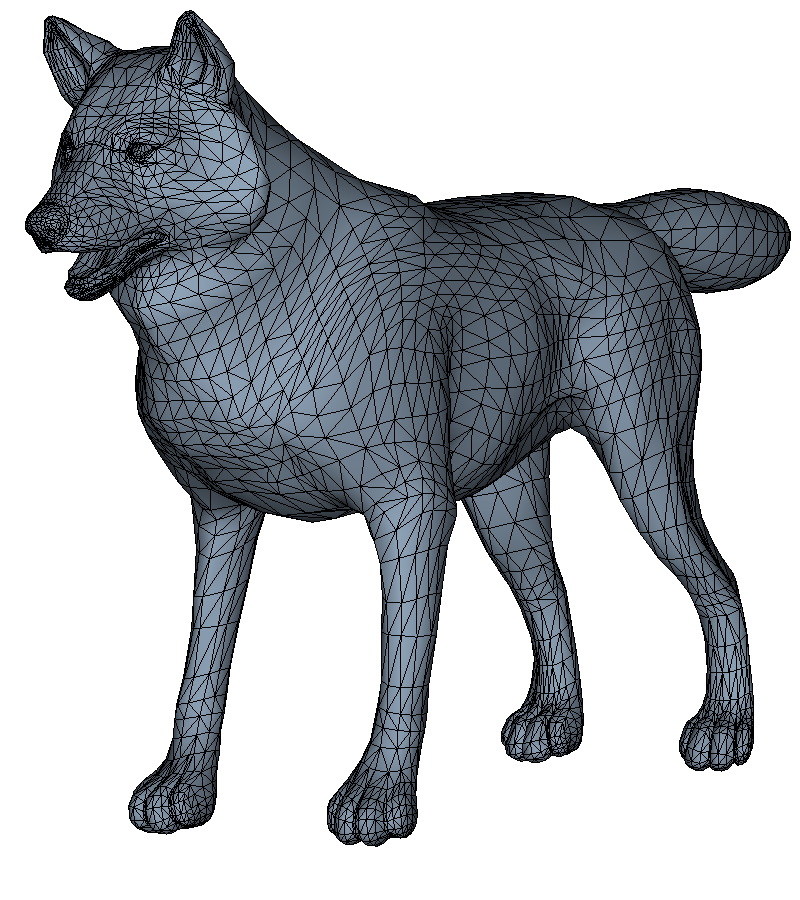
\includegraphics[width=\linewidth]{FIG34}
        \caption{}
    \end{subfigure}%
    ~
    \begin{subfigure}[b]{0.35\linewidth}
        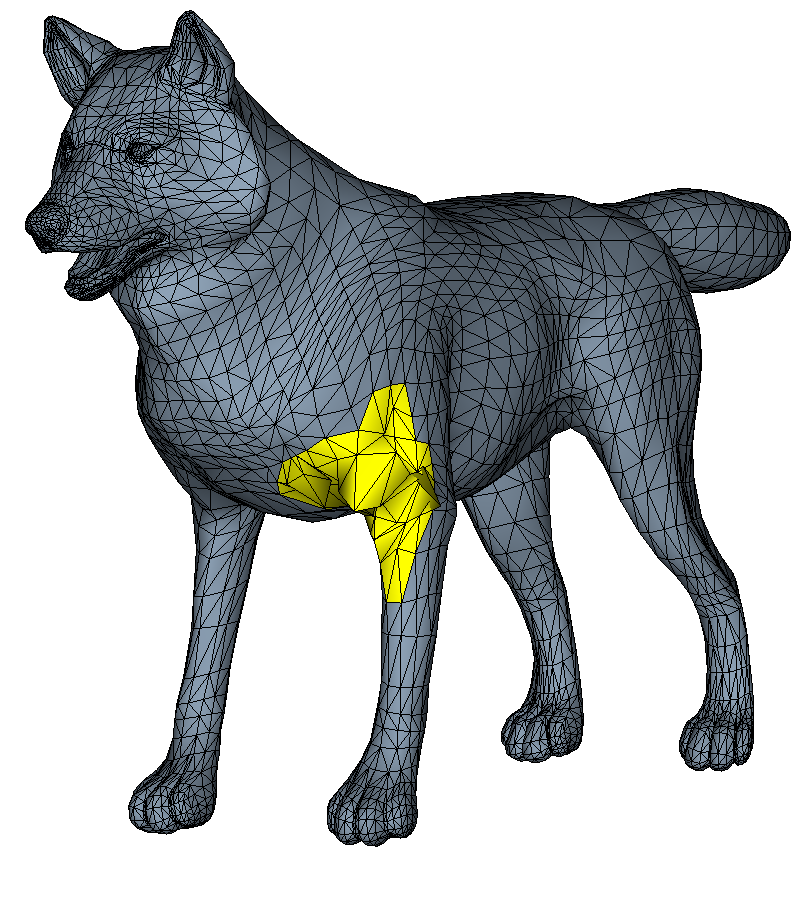
\includegraphics[width=\linewidth]{FIG35}
        \caption{}
    \end{subfigure}
    \\
    \begin{subfigure}[b]{0.35\linewidth}
        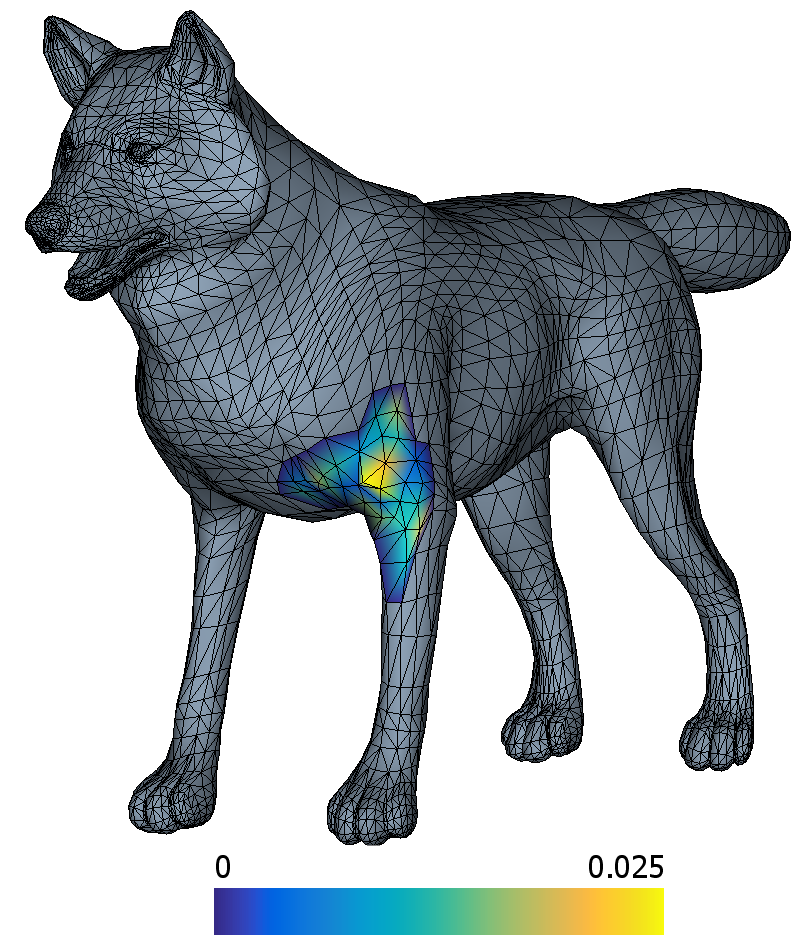
\includegraphics[width=\linewidth]{FIG36}
        \caption{}
    \end{subfigure}
    ~
    \begin{subfigure}[b]{0.35\linewidth}
        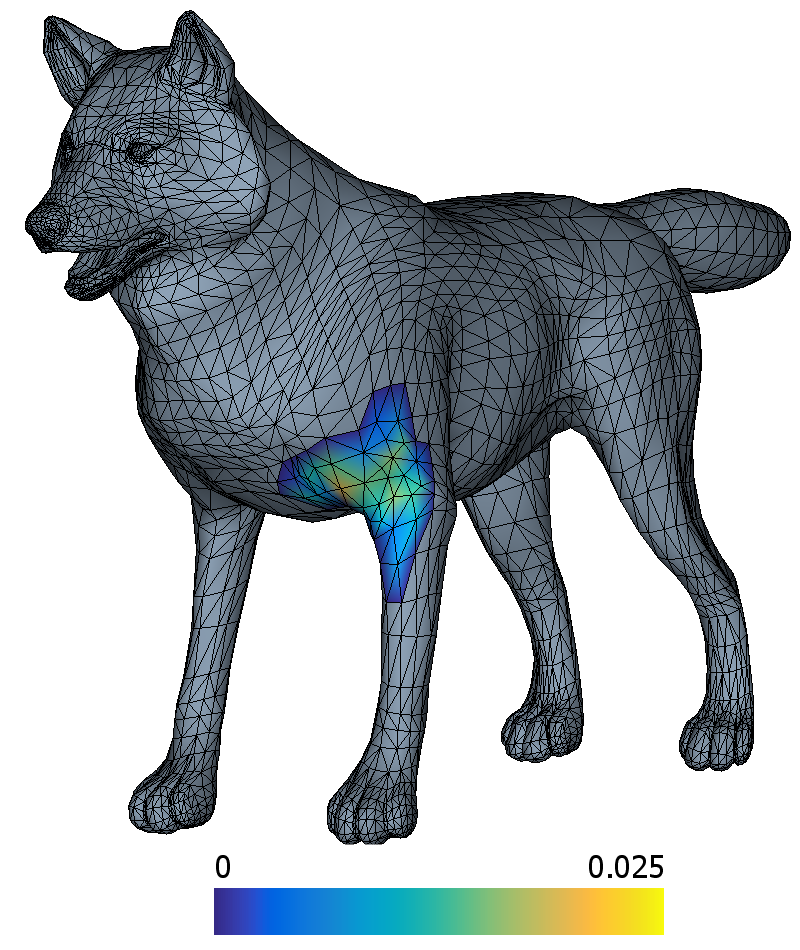
\includegraphics[width=\linewidth]{FIG37}
        \caption{}
    \end{subfigure}
    \caption[Geometry repair of the damaged wolf model.]
    {Geometry repair of the damaged wolf model.
         (a) The original wolf model; (b) Damaged model with significant noise in the region marked in yellow;
         (c) Repaired with Laplacian regularized least square smoothing~\cite{Nealen2006};
         (d) Repaired with our inpainting method. In (c) and (d), the per-vertex inpainting error (compared with the ground truth)
          is color-coded. }
\label{fig:repair:wolf}
\end{figure}

Fig.~\ref{fig:repair:cube}, \ref{fig:repair:epcot}, and \ref{fig:repair:wolf}
demonstrate repairing damaged local geometry using our sparsity-regularized
inpainting method. The results are compared with two geometry-regularized mesh
optimization methods: Laplacian regularized least square
smoothing~\cite{Nealen2006} and thin-plate energy minimization~\cite{Bac2008}.
We can see that, although geometry-regularized methods can generate patches
that are smooth and blend well with the surroundings, they fail to recognize
the intrinsic structures of the original shapes; consequently, important
geometric features are simply smoothed out. In contrast, our
sparsity-regularized inpainting method takes into account the global shape
structures, and almost perfectly recovers the edges and corners in the cube
model (Fig.~\ref{fig:repair:cube}) and the geometric textures of the epcot
model (Fig.~\ref{fig:repair:epcot}) from partial observations.


\subsection{Hole Filling}

As introduced in Sec.~\ref{sec:inpaint:holefilling}, for general hole filling
tasks, the mesh connectivity information inside holes are probably unknown. We
must first triangulate holes in a proper way and then apply our geometry
inpainting method to optimize the newly inserted mesh. How the hole is
triangulated directly impacts the global Laplacian eigenbasis which subsequently
determine the estimated recovery.

As an example, Fig.~\ref{fig:holefilling1} compares the results of filling the
holes of a double torus model with and without original connectivity
information, using our sparsity-regularized method and the geometry-regularized
method proposed in \cite{Bac2008}. We can see that estimating with a different
connectivity significantly alters the final hole fairing results. In this
example, our method generate shapes that are more approximate to the original
shape both with the original connectivity and with the new connectivity.

\begin{figure}
\centering
    \begin{subfigure}[b]{0.3\linewidth}
    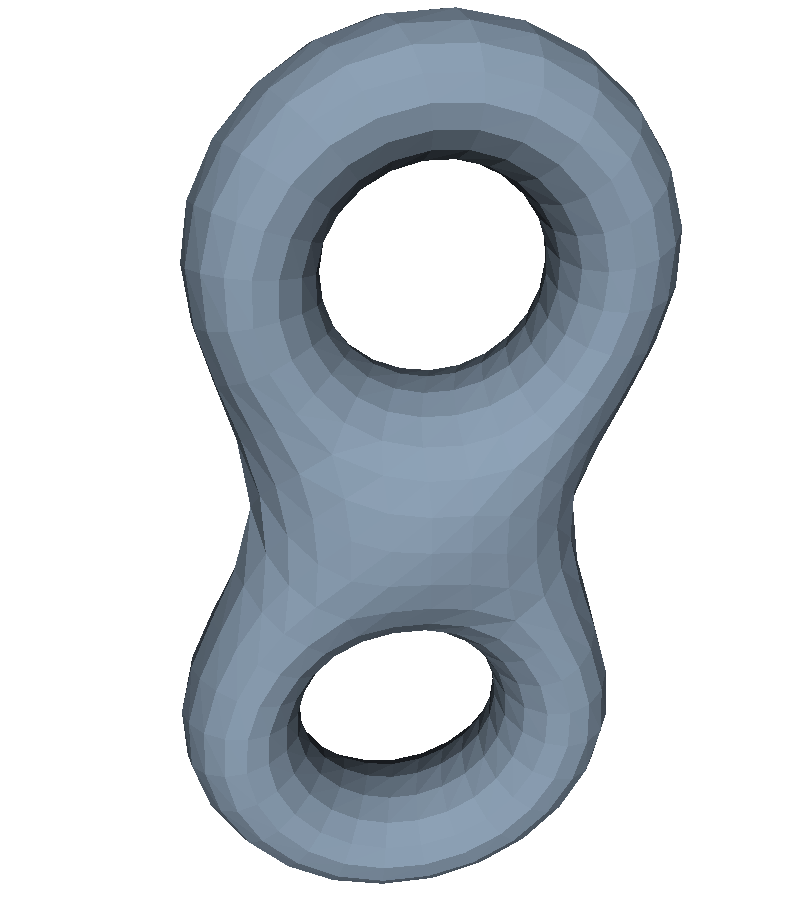
\includegraphics[width=\linewidth]{FIG38}
    \caption{}
    \end{subfigure}
    ~
    \begin{subfigure}[b]{0.3\linewidth}
    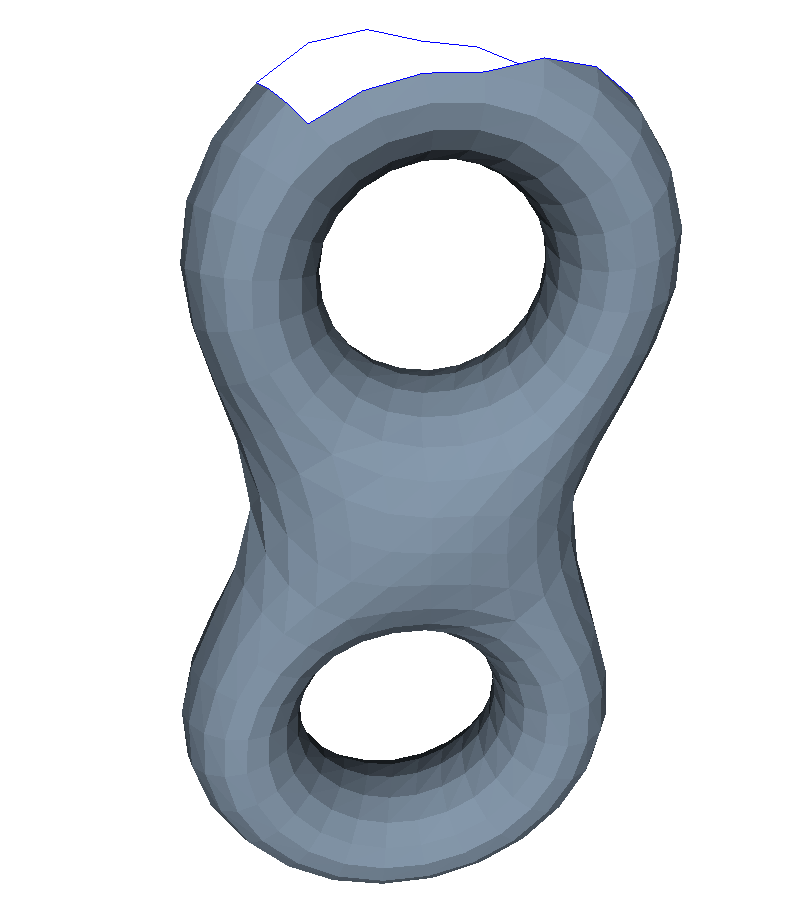
\includegraphics[width=\linewidth]{FIG39}
    \caption{}
    \end{subfigure}
    ~
    \begin{subfigure}[b]{0.3\linewidth}
    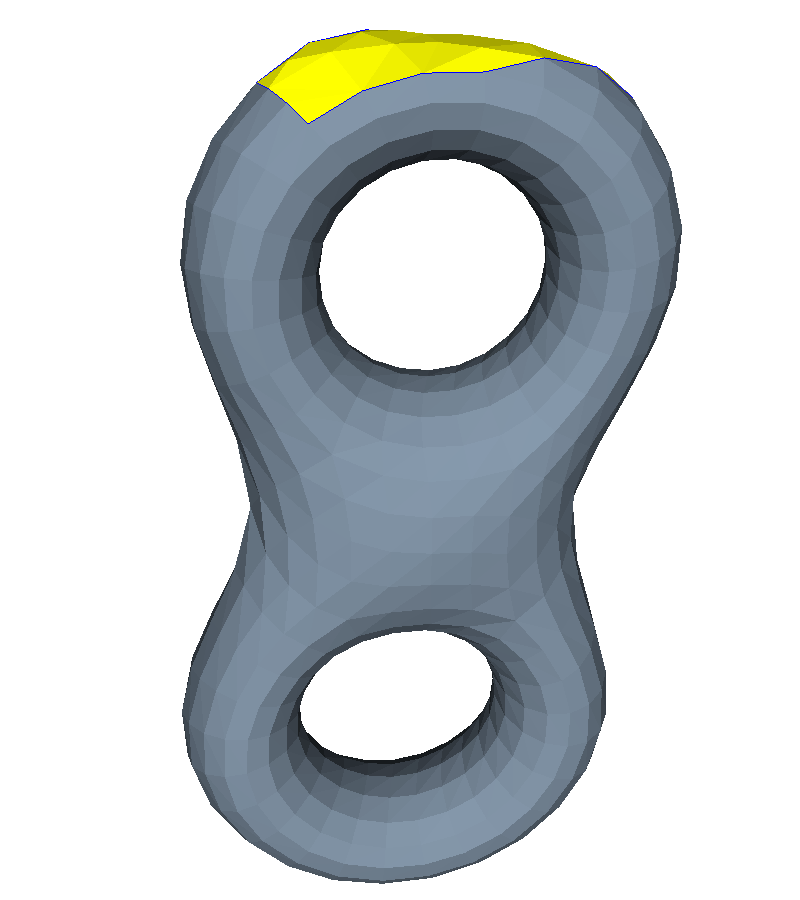
\includegraphics[width=\linewidth]{FIG40}
    \caption{Error: 0.010}
    \end{subfigure}
    \\
    \begin{subfigure}[b]{0.3\linewidth}
    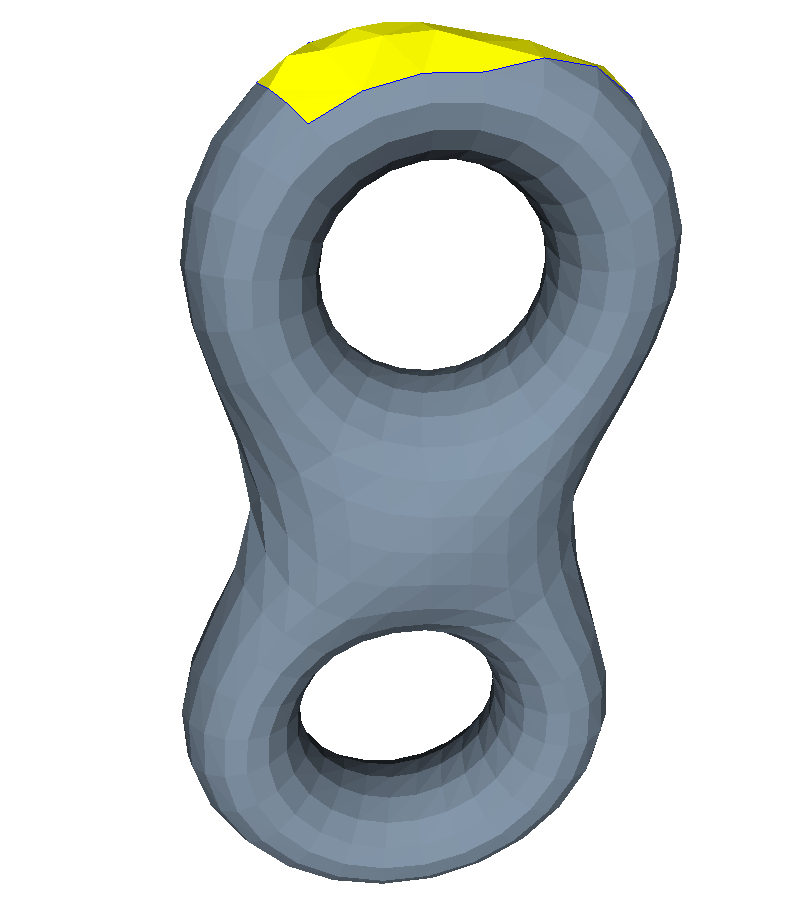
\includegraphics[width=\linewidth]{FIG41}
    \caption{Error: $4.1\times 10^{-4}$}
    \end{subfigure}
    ~
    \begin{subfigure}[b]{0.3\linewidth}
    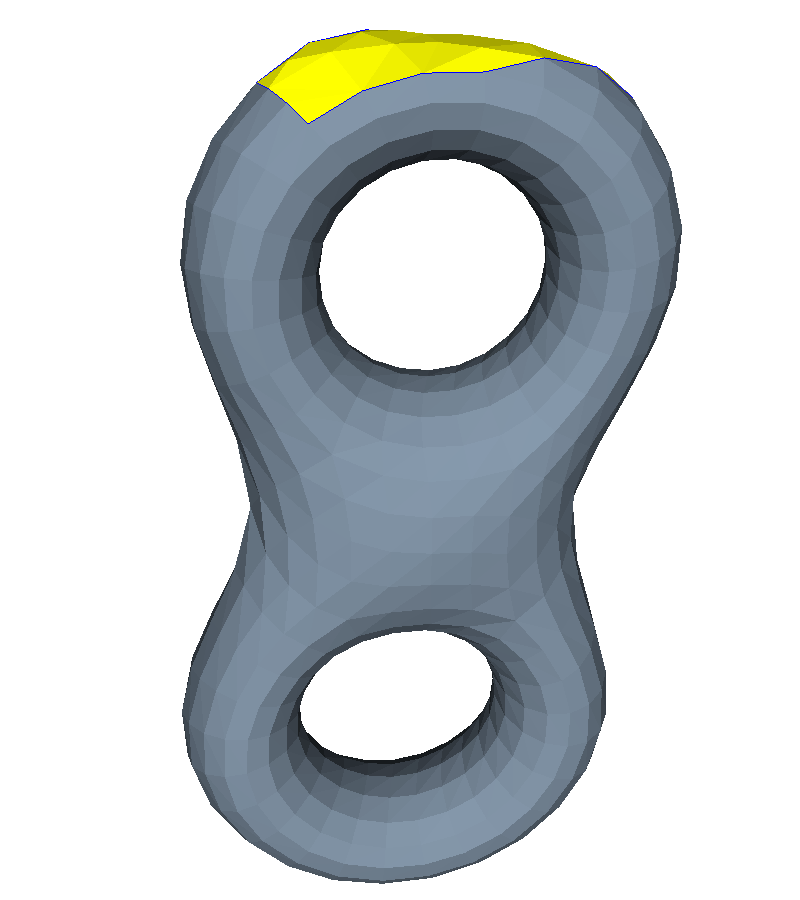
\includegraphics[width=\linewidth]{FIG42}
    \caption{Error: 0.030}
    \end{subfigure}
    ~
    \begin{subfigure}[b]{0.3\linewidth}
    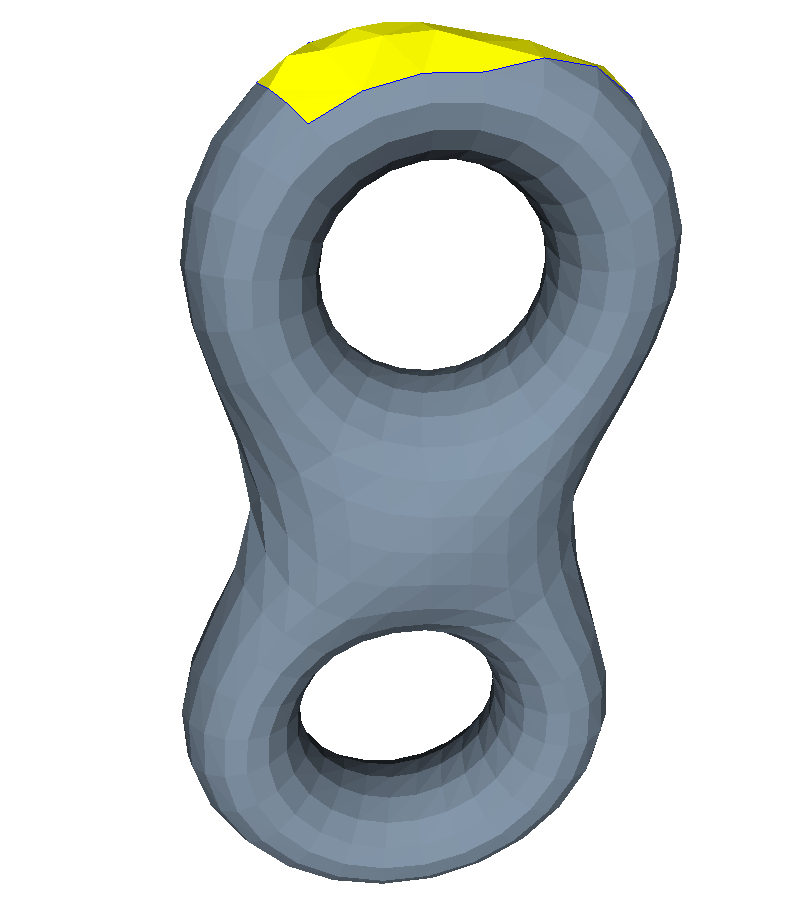
\includegraphics[width=\linewidth]{FIG43}
    \caption{Error: 0.021}
    \end{subfigure}
\caption[Comparison of hole filling results using sparsity-regularized method and geometry-regularized method.]
        {Compare hole filling results using our sparsity-regularized method and the geometry-regularized method introduced in ~\cite{Bac2008}.
        The error is measured as the root-mean-squared deviation from the estimated vertices to the original shape.
        (a) The original double torus model.
        (b) The model with a hole.
        (c) Inpainted using the method in \cite{Bac2008} with the original mesh connectivity.
        (d) Inpainted using our method with the original mesh connectivity.
        (e) Inpainted using the method in \cite{Bac2008} with the mesh connectivity generated from hole triangulation and refinement.
        (f) Inpainted using our method with the same mesh connectivity as (e).}

\label{fig:holefilling1}
\end{figure}

In general cases, we cannot expect the hole filling result using our
sparsity-regularized inpainting method to precisely match the original shape
when the number of vertices and connectivity of the patching mesh, generated
from hole triangulation and refinement, are different from the original mesh.
Nonetheless, the resulting patching meshes tend to be coherent with the whole
remaining shape, thanks to the global shape awareness of our method.
Fig.~\ref{fig:holefilling2} shows two examples of filling holes utilizing our
inpainting method. The results are comparable to the geometry-regularized
surface restoration method in \cite{Bac2008}.

\begin{figure}
\centering
    \begin{subfigure}[b]{0.33\linewidth}
        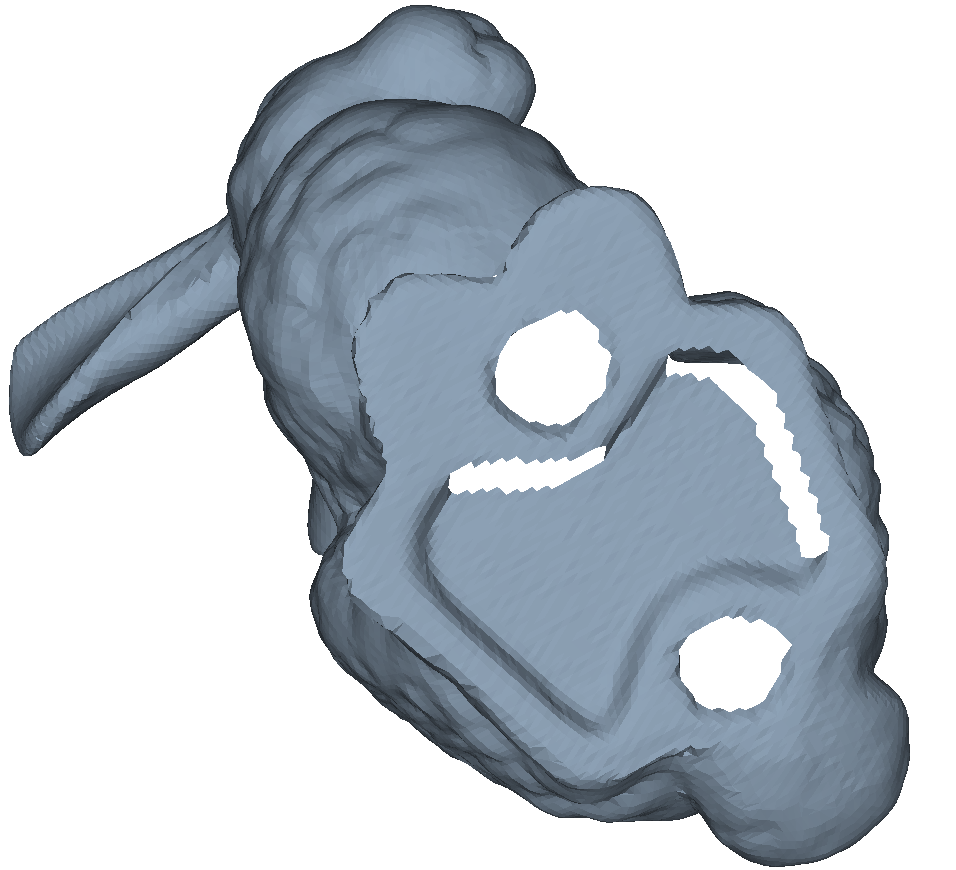
\includegraphics[width=\linewidth]{FIG44}
        \caption{}
    \end{subfigure}%
    ~
    \begin{subfigure}[b]{0.33\linewidth}
        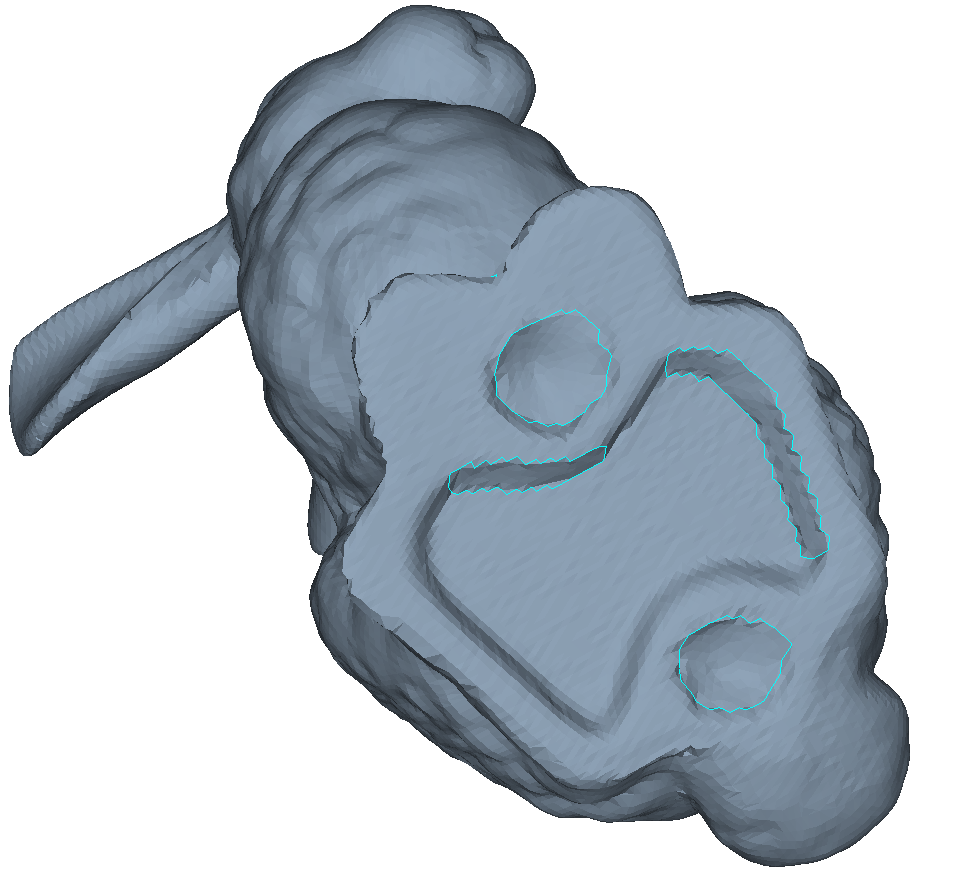
\includegraphics[width=\linewidth]{FIG45}
        \caption{}
    \end{subfigure}%
    ~
    \begin{subfigure}[b]{0.33\linewidth}
        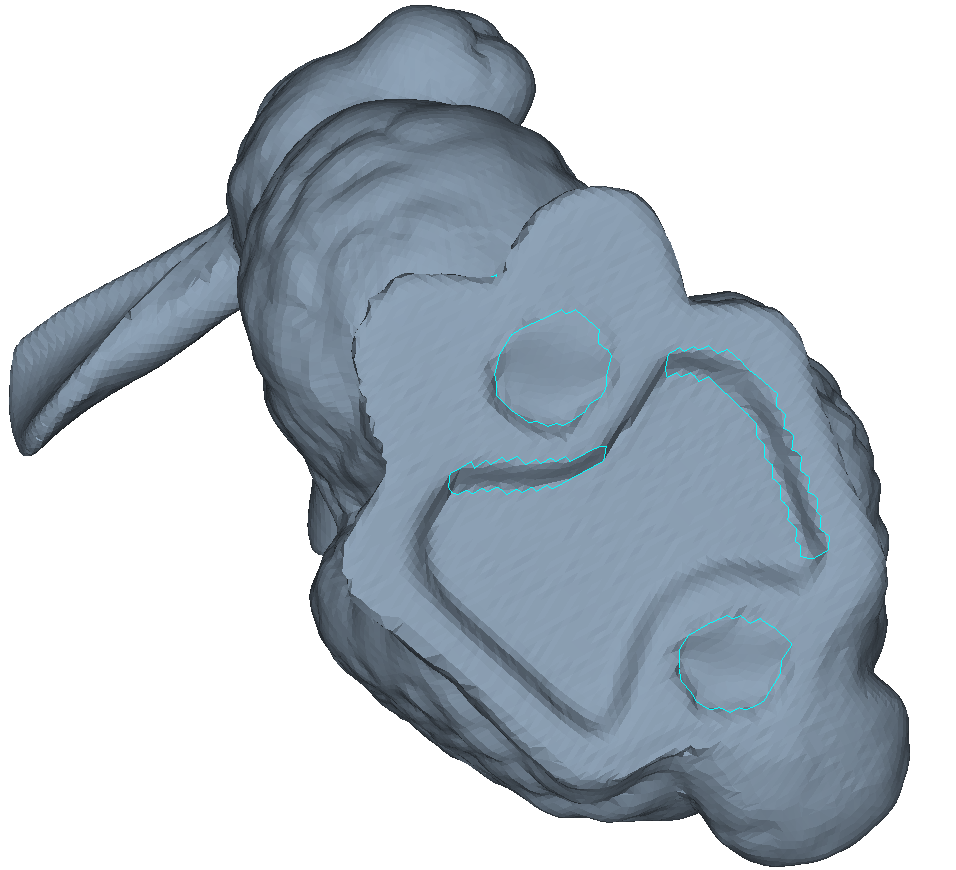
\includegraphics[width=\linewidth]{FIG46}
        \caption{}
    \end{subfigure}
    \\
    \begin{subfigure}[b]{0.33\linewidth}
        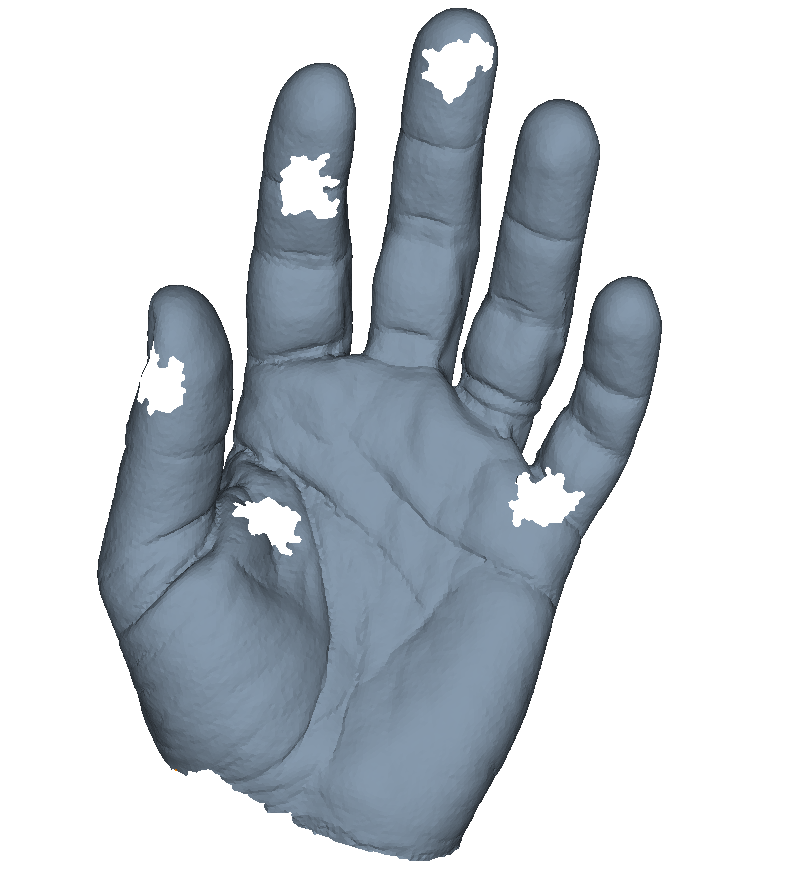
\includegraphics[width=\linewidth]{FIG47}
        \caption{}
    \end{subfigure}%
    ~
    \begin{subfigure}[b]{0.33\linewidth}
        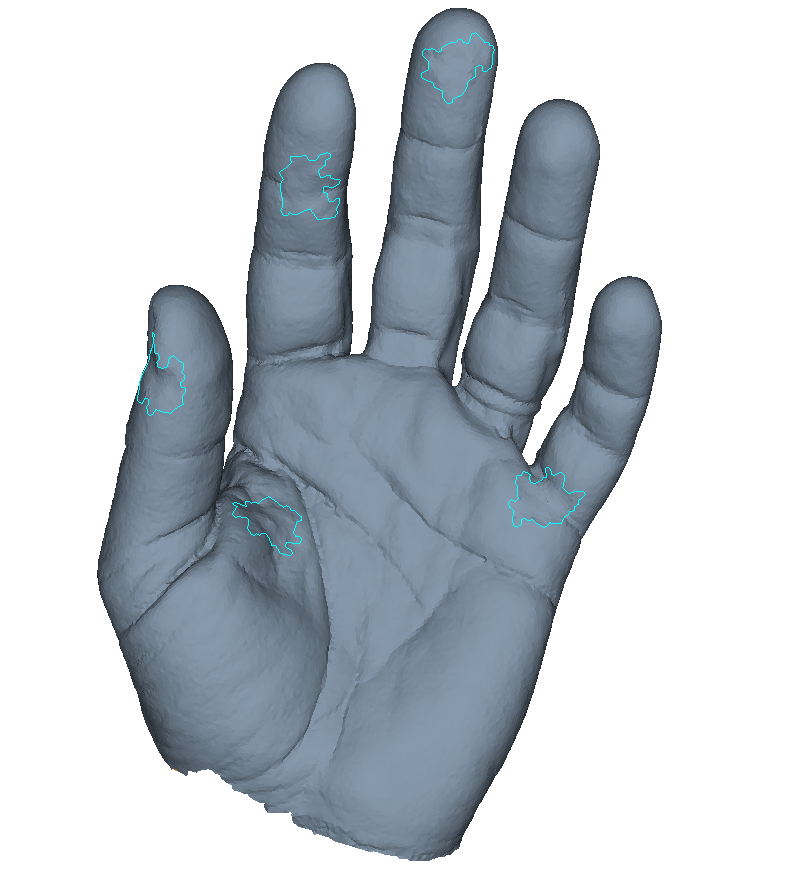
\includegraphics[width=\linewidth]{FIG48}
        \caption{}
    \end{subfigure}%
    ~
    \begin{subfigure}[b]{0.33\linewidth}
        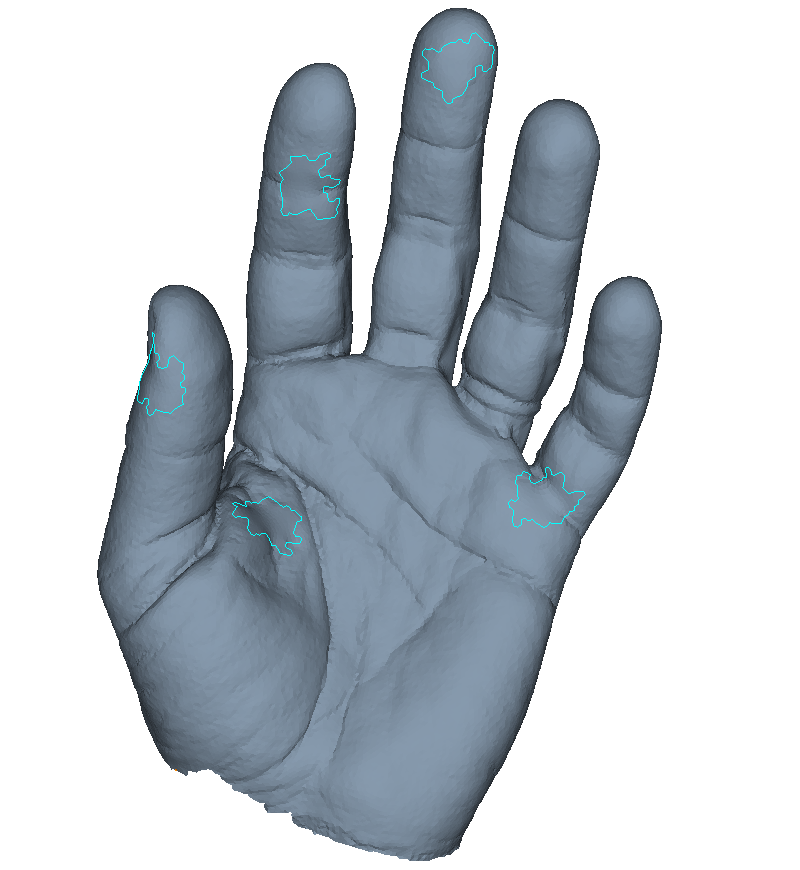
\includegraphics[width=\linewidth]{FIG49}
        \caption{}
    \end{subfigure}
\caption[Hole inpainting on the bunny and hand models.]
        {Inpainting existing holes on the bunny and hand models. (a)(d) Original models with holes;
        (b)(e) Hole-filling result using our method;
        (c)(f) Hole-filling result using the method of \cite{Bac2008}.}
\label{fig:holefilling2}
\end{figure}

\section{Chapter Summary}
In this chapter, we have proposed a novel surface inpainting algorithm based on
sparse signal recovery. Instead of directly estimating the local missing
geometry, our new inpainting framework is designed to discover the coefficient
representation of the entire original shape in a transform domain. When the
shape geometry is sufficiently sparse with respect to the dictionary of
transform basis, chances are we can accurately recover this sparse
representation by imposing sparsity constraints on the coefficients given
partial observations. In our method, we adopt the mesh Laplacian eigenbasis as
dictionary, and formulate surface inpainting as a sparse signal recovery
problem. Leveraging standard $l_1$ optimization techniques, we can obtain an
estimated shape which agrees with the observable parts and are globally
coherent. For shapes that are highly compressible w.r.t. the Laplacian
eigenbasis, we have experimentally demonstrated the great potential of our
method for geometry restoration, geometry repair, and hole filling.

For the future work, we plan to extend our sparsity-based inpainting framework
by integrating geometric constraints such as curvatures and normals, which
should improve the geometric consistency of the inpainting result. We are also
interested in designing new types of shape basis and exploring more
sophisticated strategies for constructing dictionaries, e.g., dictionaries that
are adaptive to the input shape. 